\chapter{Revisiting SATzilla Features in 2024}\label{ch:ch04:rev_SATzilla}

\section{Introduction}
\label{sec:ch04:intro}

The Boolean satisfiability problem (SAT) is an important problem in computer science from both theoretical and practical viewpoints.
Common usages of SAT include hardware and software verification, cryptography, and more.
However, as SAT is $\mathcal{NP}$-complete, it takes substantial time and computing power to solve it, which becomes prohibitively expensive as formulas become larger.
In order to deepen our understanding of SAT itself and develop better SAT solvers, it is of crucial importance to be able to describe SAT instances via an informative set of features.

Some of the most widely adopted such features are the SATZilla features~\cite{NudEtAl04,HutEtAl14}.
These are a fixed set of features that are calculated from the DIMACS CNF representation of a SAT instance. The SATZilla features consist of multiple groups, ranging from basic syntactic features describing the formula, such as its number of variables and clauses, to more complicated features, such as probing features derived from short runs of SAT solvers. Another type of features are based on statistics of graph representations of a given formula.

The SATZilla features have been successfully used in various domains, such as empirical performance models (EPMs; also known as performance or running time prediction) and algorithm selection~\cite{XuEtAl08,XuEtAl12}, algorithm configuration~\cite{HutEtAl11}, and benchmark generation~\cite{LeyEtAl09}.
The features are also used for caching in CDCL-based model counting solvers~\cite{RooEtAl21} and in a variety of SAT solvers that incorporate machine learning techniques~\cite{GuoEtAl23}
However, the SATZilla features in their latest version date back to 2012.
Since then, the SAT community has undergone various changes.
Most notably, SAT instances that we typically encounter today have a larger number of variables and clauses, thus taking significantly more time and memory to preprocess. Currently, the existing SATZilla feature extraction tool is unable to compute many of these features because of time and memory limitations.

In this paper, we revisit the SATZilla features and introduce a new version of the feature extraction tool. First, we replace the underlying solvers and the preprocessor with their most up-to-date versions. We then fix compilation errors and other memory errors related to dealing with larger formulas. Finally, we allow the user to set the time limits for feature computation.
We compare the performance of our new tool with the old one in two SAT competitions. We measure the running times and the number of extracted features to check for performance gains of our new tool. We then evaluate the extracted features on three downstream tasks: satisfiability prediction, performance prediction and algorithm selection. We show that our new tool yields an important advantage in performance compared to the old tool across all three tasks.

The rest of the paper is organised as follows. We give a historical overview of the development and applications of the SATZilla features in~\cref{sec:ch04:related-work}. We then introduce the technical definitions, as well as the standard methodological pipeline in~\cref{sec:ch04:satzilla-features}, wrapping it up with the contributions of this study. The results are presented in~\cref{sec:ch04:experiments}, and conclusions drawn in~\cref{sec:ch04:conclusions}.

\section{Related work}
\label{sec:ch04:related-work}

The SATZilla features were first introduced by Nudelman~et~al.~\cite{NudEtAl04} to construct EPMs, \emph{i.e.}, machine learning models that predict the running time of various SAT solvers given the features representing SAT instances. The authors identified key features that contribute the most towards having a good EPM prediction.
Consequently, they used the EPMs as a basis for algorithm selection, in which the algorithm that is selected corresponds to the one with the lowest predicted running time.
They leveraged the \textit{performance complementarity} phenomenon of SAT solvers, where no SAT solver dominates all others over all instances.
Therefore, selecting the best solver for each instance results in substantially better performance compared to choosing any standalone solver for all instances.
The SATZilla features were also successfully used for the satisfiability prediction task for SAT instances from various distributions~\cite{DevOSu08}.

Further developments in algorithm selection led to the 2007 version of the SATZilla algorithm selector~\cite{XuEtAl08}, which combined running time and satisfiability prediction with other improvements. It won multiple medals in the SAT competition. This shows that extracting features from SAT instances can also speed up the solving process, and not only help understanding SAT. A newer version of the SATZilla algorithm selector was introduced in 2012~\cite{XuEtAl12}, winning multiple awards as well. It used a random forest as a predictor, and introduced an ensemble of pairwise classifiers to establish a ranking of the solvers, instead of predicting the running times directly. Additional features were introduced thereafter, revealing further important information about SAT instances.

Another common usage of the SATZilla features is (model-based) algorithm configuration. To this end, the hyperparameters of SAT solvers are optimised such that their performance is as good as possible on all instances. As running SAT solvers is computationally expensive, a surrogate model is employed; it takes as an input a configuration of hyperparameters and instance features and predicts the performance of the SAT solver using a given configuration on a given instance. The instance features boost the accuracy of the surrogate model. An example of that is SMAC~\cite{HutEtAl11}, which successfully used the SATZilla features to optimise the performance of a wide range of SAT solvers on various benchmarks.

Last but not least, feature-based EPMs are proven to be useful for benchmark generation~\cite{LeyEtAl09}. In this context, given a new instance, we compute the features, which is usually cheaper than running a SAT solver, and use the EPM to predict whether the instance is hard (or not) for the solvers at hand.

\section{SATZilla features}
\label{sec:ch04:satzilla-features}

The SATZilla features describe the SAT formula using various representations and statistics. Their graph-based features summarise the variable graph (VG), clause graph (CG), and variable-clause graph (VCG) defined in~\cref{sec:ch03:sat-graphs}, using statistics such as node degrees, clustering coefficients, and graph diameter.

Feature computation starts with the \emph{preprocessing} of the formula. This step, performed before solving an instance, renders the formula more accessible for SAT solvers. This means that the features are also computed on the version of the formula that is close to the one seen by the solvers. We believe that all these aspects can be boosted by using a modern preprocessor.
Features are classically computed using the \textsc{SATElite} preprocessor. We instead use the SBVA preprocessor, suggested by the winning solver from the 2023 SAT Competition. SBVA is also able to terminate after a set cutoff time, allowing for partial preprocessing, while \textsc{SATElite} does not include this functionality.
The preprocessed formula can subsequently be passed to a SAT solver, although the solver may still apply its own preprocessing and inprocessing procedures. Reusing this formula can avoid repeating external preprocessing; it does not imply that all portfolio solvers operate on exactly the same internal representation.

Preprocessing is also part of the definition of the feature representation. It preserves satisfiability, but can change the number of variables and clauses, their incidence patterns, and the behaviour observed during probing. Thus, two preprocessors can produce different feature vectors for the same original instance. When preprocessing succeeds, the features below characterise the resulting representation, apart from the preliminary descriptors of the original formula. If preprocessing fails, the external clause-learning and local-search probes fall back to the original input. Smaller representations need not be easier to solve, and a transformation that helps a solver need not make graph-based feature extraction cheaper.

Following the preprocessing, the \emph{feature extraction} begins. We describe eleven feature groups, counting local search as one group containing two separately timed solver probes. This gives twelve timing blocks in the computation-time figures. We describe the groups according to their implementation in the SATZilla feature extraction tool, rather than the grouping in the corresponding paper~\cite{HutEtAl14}. The feature counts below include the computation-time feature for each block.

The groups provide complementary views of an instance: syntactic and graph-based features describe its representation, whereas probing features describe the response of a particular search procedure to that representation. Many features summarise a distribution over variables, clauses, or probe runs. The mean describes a typical value, while the minimum, maximum, dispersion, and quantiles reveal heterogeneity that an average alone would conceal. For example, two formulas can have the same average variable occurrence count, but differ in whether occurrences are spread evenly or concentrated around a few variables. The coefficient of variation expresses standard deviation relative to the mean, where defined, and entropy summarises the diversity of the recorded values. These summaries are predictive descriptors, rather than guarantees of satisfiability or solving difficulty.

\noindent\textbf{Preliminary} features include the number of variables and clauses before and after preprocessing, together with their relative reductions. They describe both the original scale of an instance and how strongly the preprocessor transforms it. The running time of this feature group includes preprocessing and reading the formula. This group contains 7 features.

\noindent\textbf{Basic} features are cheap features that describe clause size and polarity balance, together with the variable-clause ratio. Clause-node degrees in the VCG correspond to the number of variables occurring in each clause. The implementation records the fraction of unary clauses and the cumulative fractions of clauses of length at most two and at most three, rather than three separate clause counts. Short clauses restrict fewer variables at a time and can become unit clauses after fewer assignments. Polarity-balance statistics distinguish clauses with similar numbers of positive and negative literals from clauses dominated by one polarity. Together, these features describe local constraint structure beyond the overall formula size. This group contains 15 features.

\noindent\textbf{KLB} features include variable-node degree statistics in the VCG and VG, variable polarity balance, and proximity to a Horn formula. VCG degrees describe how often variables occur, while VG degrees describe how many other variables they share clauses with. Their distributions distinguish broadly distributed interactions from concentrations around highly connected variables. Polarity balance measures whether a variable occurs comparably often in both polarities or predominantly in one. A Horn clause has at most one positive literal; the group records the fraction of such clauses and statistics on each variable's occurrences in them. These are syntactic measures of Horn-like structure, rather than a guarantee that the entire formula belongs to that tractable class. Constructing variable neighbourhoods makes this group more expensive than the basic features. This group contains 21 features.

\noindent\textbf{Clause graph} (CG) features contain statistics on node degrees and clustering coefficients in the clause graph. Degrees describe how many other clauses each clause is connected to, and clustering describes how densely its neighbours are connected to one another. They therefore characterise local concentrations of interacting constraints. Explicitly constructing these neighbourhoods can be expensive even when the input CNF has a compact representation. This group contains 11 features.

\noindent\textbf{Diameter} features summarise distances in the variable graph. For a node $v$, its eccentricity within its connected component is $e(v)=\max_{u\in\mathcal{C}(v)}d(v,u)$, where $d(v,u)$ is the shortest-path distance and $\mathcal{C}(v)$ is the component containing $v$. The diameter of a connected graph is the maximum eccentricity, rather than an individual shortest-path distance. The extractor aggregates traversal depths over source variables using the mean, coefficient of variation, minimum, maximum, and entropy. Its breadth-first traversal counts the source at depth one, so the recorded depths are one larger than the corresponding edge distances; unreachable components are not traversed from that source. These features describe how far interactions extend through chains of co-occurring variables. This group contains 6 features.

\noindent\textbf{DPLL probing} (or unit propagation) features are computed by making tentative assignments and measuring the additional variables fixed by unit propagation at decision depths 1, 4, 16, 64, and 256. The reported reductions are normalised by the number of variables and exclude the explicit decisions themselves. A large reduction indicates that a small number of decisions triggers many implications under the probing procedure. It does not by itself establish that a complete solver will find a solution or a refutation quickly. This group contains 6 features.

\noindent\textbf{Lobjois} features estimate search-space size from repeated randomised DPLL probes. The extractor records a mean terminal depth and a separate log-scale estimate based on averaging $2^{d_r}$ over probe depths $d_r$, then taking the base-two logarithm. Both depth descriptors are normalised by the number of variables. The logarithm of this average is not generally the average depth: deeper probes have a larger influence on the search-space estimate. These features characterise the search tree encountered by the probing procedure, rather than directly measuring the work of a modern CDCL solver. This group contains 3 features, including timing, and is based on the work of Lobjois and Lema\^{\i}tre~\cite{LobLem98}.

\noindent\textbf{Survey propagation} features summarise approximate variable-bias information returned by VARSAT~\cite{HsuMcI09}. The underlying quantities estimate whether each variable is forced towards True, forced towards False, or unconstrained across satisfying assignments. The extractor summarises polarity confidence and the estimated unconstrained probability over variables. These features describe the inferred organisation of the solution space, complementing purely syntactic polarity counts. They are estimates from an inference procedure, not certified statements about forced assignments or satisfiability. This group contains 19 features.

\noindent\textbf{Clause learning} (CL) features are based on short runs of a CDCL solver (ZChaff rand~\cite{MahEtAl04} in the 2012 version, CaDiCaL~\cite{BieEtAl20} in our new version). We measure the number and length of learned clauses at intervals of 1000 decisions and summarise those observations. The features describe early conflict-driven search behaviour: how frequently the probe learns clauses and how large those clauses are. Their values depend on the probing solver and its search policy as well as on the formula; replacing the solver can therefore change their predictive content. This group contains 19 features.

\noindent\textbf{Local search} (LS) features are obtained from repeated runs of GSAT and a second stochastic local search solver: SAPS in the 2012 version and Sparrow 2011 in our new version. Each probe is configured for up to 10000 runs under a two-second global search budget per solver; 10000 is a run count, not a per-run step limit. The recorded statistics describe the smallest number of unsatisfied clauses reached, the steps to the first local minimum, the average improvement towards the best value, and the fraction of the total improvement achieved on reaching the first local minimum. Means, coefficients of variation, and selected quantiles across runs describe both progress and variability. These observations reveal how readily the chosen procedure improves assignments and whether it stagnates, without certifying unsatisfiability when no solution is found. Each solver contributes 11 search statistics and one timing feature, giving 24 features in total. The second block retains the historical \texttt{saps} column names when Sparrow is used; accordingly, the timing figures label it SAPS/Sparrow. Identical column names across versions do not imply identical probing behaviour.

\noindent\textbf{Linear programming} (LP) features are based on a continuous relaxation of the preprocessed formula $C_1\land\cdots\land C_N$ over Boolean variables $x_j$. Replacing Boolean variables by real variables in $[0,1]$, define $v(x_j)=x_j$ and $v(\neg x_j)=1-x_j$, and solve
\begin{equation*}
    \begin{aligned}
        \text{maximise}\quad & \sum_{i=1}^{N}\sum_{\ell\in C_i}v(\ell) \\
        \text{subject to}\quad & \sum_{\ell\in C_i}v(\ell)\geq 1, \qquad i=1,\ldots,N, \\
        & 0\leq x_j\leq 1 \qquad\text{for every variable }x_j.
    \end{aligned}
\end{equation*}
For Boolean assignments, each clause constraint requires at least one true literal. Allowing fractional values gives a relaxation: a satisfying Boolean assignment is feasible, but a feasible fractional solution need not correspond to a satisfying assignment. The objective favours a large total literal value; it does not count satisfied clauses. The implementation omits the constant contribution of negative literals from the objective and divides the resulting objective value by $N$ when reporting \texttt{LP\_OBJ}. The remaining descriptors summarise the distances $\min(x_j,1-x_j)$ to the nearest Boolean value and the fraction of variables with integral values. They describe how fractional the returned optimum is, rather than providing a general test for satisfiability. In the new version, we upgrade the LP solver package, lp\_solve. This group contains 7 features, including timing.

We note that the basic, KLB and clause graph features are computed sequentially, with each feature group being dependent on the successful computation of the previous groups; \emph{e.g.}, if the computation of the basic features fails, the KLB and clause graph features will not be computed at all.

Another change we applied to the feature extraction tool is allowing a more precise timeout setting. In the 2012 version, the time limits were hard-coded and set to high values (for example, 1200 seconds for preprocessing). This can cause many feature computations to simply terminate without computing any features at all. To this end, we adjust the code in the new version to allow the user to set the time limits through a command line argument.

\section{Experiments}
\label{sec:ch04:experiments}
We evaluate our new SATZilla feature extraction tool on the formulas stemming from two latest (2022 and 2023) SAT Competitions. We first look at the feature extraction times and then evaluate the features on three downstream tasks: satisfiability prediction, running time prediction, and algorithm selection.
To assess the advantage of using the new version of the extraction tool, we extract the features using both our new version and the 2012 version of the tool, with a time limit of 180 seconds per feature group.

We use a cluster of 18 nodes, each equipped with 2 AMD EPYC 7543 32-core CPUs with 256 MB L3 cache. Each node also has 1TB of memory. The cluster is running on a Rocky Linux 9.4 operating system. We measure running times using the runsolver tool \cite{Roussel11c}.

\subsection{Feature computation time}
\label{sec:ch04:feature-computation-time}

\begin{figure*}[h]
    \caption[Feature computation on the 2022 SAT Competition]{Percentage of instances for which each feature block is computed within the available time budget by the old tool (SATZilla 2012; in rose) and the new tool (SATZilla 2024; in indigo) on the 2022 SAT Competition. For most feature groups, the new tool extracts features from more instances than the old one.}
    \centering
    \begin{subfigure}[b]{0.32\textwidth}
        \centering
        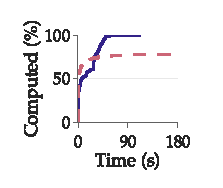
\includegraphics{figures/04/figs/ecdf_sc2022_Pre-featuretime.pdf}
        \caption{Preliminary}
        \label{fig:ch04:satcomp22_pre}
    \end{subfigure}\hfill
\begin{subfigure}[b]{0.32\textwidth}
        \centering
        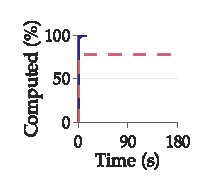
\includegraphics{figures/04/figs/ecdf_sc2022_Basic-featuretime.pdf}
        \caption{Basic}
        \label{fig:ch04:satcomp22_basic}
    \end{subfigure}\hfill
\begin{subfigure}[b]{0.32\textwidth}
        \centering
        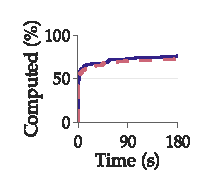
\includegraphics{figures/04/figs/ecdf_sc2022_KLB-featuretime.pdf}
        \caption{KLB}
        \label{fig:ch04:satcomp22_klb}
    \end{subfigure}
\par\medskip
\begin{subfigure}[b]{0.32\textwidth}
        \centering
        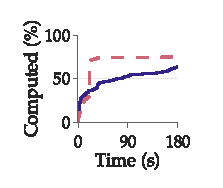
\includegraphics{figures/04/figs/ecdf_sc2022_CG-featuretime.pdf}
        \caption{Clause graph}
        \label{fig:ch04:satcomp22_cg}
    \end{subfigure}\hfill
\begin{subfigure}[b]{0.32\textwidth}
        \centering
        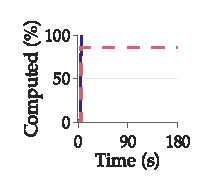
\includegraphics{figures/04/figs/ecdf_sc2022_cl-featuretime.pdf}
        \caption{Clause learning}
        \label{fig:ch04:satcomp22_cl}
    \end{subfigure}\hfill
\begin{subfigure}[b]{0.32\textwidth}
        \centering
        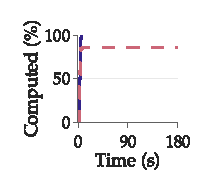
\includegraphics{figures/04/figs/ecdf_sc2022_ls-gsat-featuretime.pdf}
        \caption{LS: GSAT}
        \label{fig:ch04:satcomp22_ls_gsat}
    \end{subfigure}
\par\medskip
\begin{subfigure}[b]{0.32\textwidth}
        \centering
        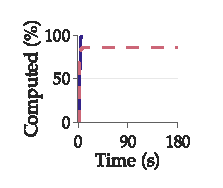
\includegraphics{figures/04/figs/ecdf_sc2022_ls-saps-featuretime.pdf}
        \caption{LS: SAPS/Sparrow}
        \label{fig:ch04:satcomp22_ls_saps}
    \end{subfigure}\hfill
\begin{subfigure}[b]{0.32\textwidth}
        \centering
        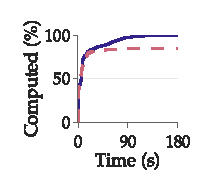
\includegraphics{figures/04/figs/ecdf_sc2022_sp-featuretime.pdf}
        \caption{Survey propagation}
        \label{fig:ch04:satcomp22_sp}
    \end{subfigure}\hfill
\begin{subfigure}[b]{0.32\textwidth}
        \centering
        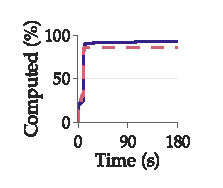
\includegraphics{figures/04/figs/ecdf_sc2022_DIAMETER-featuretime.pdf}
        \caption{Diameter}
        \label{fig:ch04:satcomp22_dia}
    \end{subfigure}
\par\medskip
\begin{subfigure}[b]{0.32\textwidth}
        \centering
        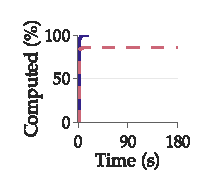
\includegraphics{figures/04/figs/ecdf_sc2022_lobjois-featuretime.pdf}
        \caption{Lobjois}
        \label{fig:ch04:satcomp22_lobjois}
    \end{subfigure}\hfill
\begin{subfigure}[b]{0.32\textwidth}
        \centering
        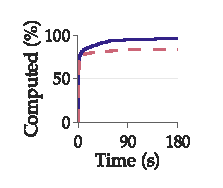
\includegraphics{figures/04/figs/ecdf_sc2022_unit-featuretime.pdf}
        \caption{Unit propagation}
        \label{fig:ch04:satcomp22_unit}
    \end{subfigure}\hfill
\begin{subfigure}[b]{0.32\textwidth}
        \centering
        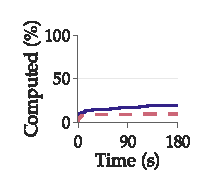
\includegraphics{figures/04/figs/ecdf_sc2022_lpTIME.pdf}
        \caption{Linear programming}
        \label{fig:ch04:satcomp22_lp}
    \end{subfigure}

    \label{fig:ch04:feat_comtimes_2022}
\end{figure*}

\begin{figure*}[h]
    \caption[Feature computation on the 2023 SAT Competition]{Percentage of instances for which each feature block is computed within the available time budget by the old tool (SATZilla 2012; in rose) and the new tool (SATZilla 2024; in indigo) on the 2023 SAT Competition. For most feature groups, the new tool extracts features from more instances than the old one.}

    \begin{subfigure}[b]{0.32\textwidth}
        \centering
        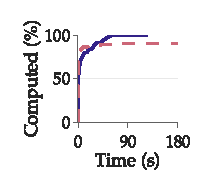
\includegraphics{figures/04/figs/ecdf_sc2023_Pre-featuretime.pdf}
        \caption{Preliminary}
        \label{fig:ch04:satcomp23_pre}
    \end{subfigure}\hfill
\begin{subfigure}[b]{0.32\textwidth}
        \centering
        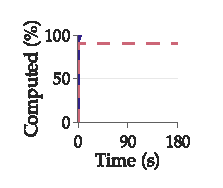
\includegraphics{figures/04/figs/ecdf_sc2023_Basic-featuretime.pdf}
        \caption{Basic}
        \label{fig:ch04:satcomp23_basic}
    \end{subfigure}\hfill
\begin{subfigure}[b]{0.32\textwidth}
        \centering
        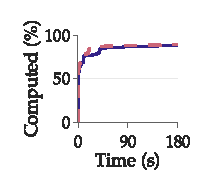
\includegraphics{figures/04/figs/ecdf_sc2023_KLB-featuretime.pdf}
        \caption{KLB}
        \label{fig:ch04:satcomp23_klb}
    \end{subfigure}
\par\medskip
\begin{subfigure}[b]{0.32\textwidth}
        \centering
        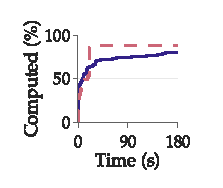
\includegraphics{figures/04/figs/ecdf_sc2023_CG-featuretime.pdf}
        \caption{Clause graph}
        \label{fig:ch04:satcomp23_cg}
    \end{subfigure}\hfill
\begin{subfigure}[b]{0.32\textwidth}
        \centering
        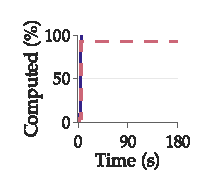
\includegraphics{figures/04/figs/ecdf_sc2023_cl-featuretime.pdf}
        \caption{Clause learning}
        \label{fig:ch04:satcomp23_cl}
    \end{subfigure}\hfill
\begin{subfigure}[b]{0.32\textwidth}
        \centering
        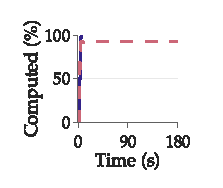
\includegraphics{figures/04/figs/ecdf_sc2023_ls-gsat-featuretime.pdf}
        \caption{LS: GSAT}
        \label{fig:ch04:satcomp23_ls_gsat}
    \end{subfigure}
\par\medskip
\begin{subfigure}[b]{0.32\textwidth}
        \centering
        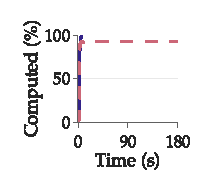
\includegraphics{figures/04/figs/ecdf_sc2023_ls-saps-featuretime.pdf}
        \caption{LS: SAPS/Sparrow}
        \label{fig:ch04:satcomp23_ls_saps}
    \end{subfigure}\hfill
\begin{subfigure}[b]{0.32\textwidth}
        \centering
        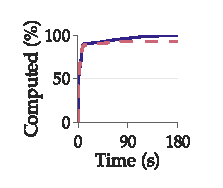
\includegraphics{figures/04/figs/ecdf_sc2023_sp-featuretime.pdf}
        \caption{Survey propagation}
        \label{fig:ch04:satcomp23_sp}
    \end{subfigure}\hfill
\begin{subfigure}[b]{0.32\textwidth}
        \centering
        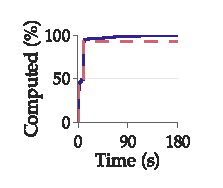
\includegraphics{figures/04/figs/ecdf_sc2023_DIAMETER-featuretime.pdf}
        \caption{Diameter}
        \label{fig:ch04:satcomp23_dia}
    \end{subfigure}
\par\medskip
\begin{subfigure}[b]{0.32\textwidth}
        \centering
        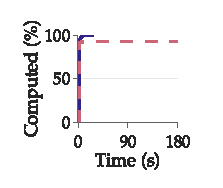
\includegraphics{figures/04/figs/ecdf_sc2023_lobjois-featuretime.pdf}
        \caption{Lobjois}
        \label{fig:ch04:satcomp23_lobjois}
    \end{subfigure}\hfill
\begin{subfigure}[b]{0.32\textwidth}
        \centering
        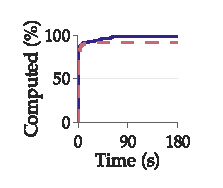
\includegraphics{figures/04/figs/ecdf_sc2023_unit-featuretime.pdf}
        \caption{Unit propagation}
        \label{fig:ch04:satcomp23_unit}
    \end{subfigure}\hfill
\begin{subfigure}[b]{0.32\textwidth}
        \centering
        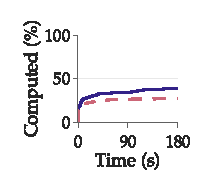
\includegraphics{figures/04/figs/ecdf_sc2023_lpTIME.pdf}
        \caption{Linear programming}
        \label{fig:ch04:satcomp23_lp}
    \end{subfigure}

    \label{fig:ch04:feat_comtimes_2023}
\end{figure*}

\cref{fig:ch04:feat_comtimes_2022,fig:ch04:feat_comtimes_2023} show, for each timing block, the fraction of instances for which computation finishes within the available time budget using the old (depicted in rose) and new (depicted in indigo) SATZilla tool on the 2022 and 2023 SAT Competition data, respectively. These curves describe feature-block availability over instances, rather than the fraction of individual feature values computed within a block. For simplicity, due to the similarity of the overall results between the two competitions, we draw more detailed insights based on plots from the 2023 edition (\cref{fig:ch04:feat_comtimes_2023}).

We first observe that the new tool is able to extract more features than the old one for most feature groups. In particular, we highlight the performance gains on the preliminary feature group (\cref{fig:ch04:satcomp23_pre}), for which the new tool can extract the features for all formulas, compared to less than $80\%$ of the formulas when using the the old tool. We note that for some feature groups, like the clause graph (\cref{fig:ch04:satcomp23_cg}), the old tool is able to extract more features compared to the preliminary feature group. This is due to the fact that the old tool extracts the preliminary, basic, KLB and CG feature groups together. Therefore, in case computing one of those groups takes a long time, the whole feature extraction fails.

We also note that for KLB and CG features there is an advantage for the old version, due to the new SBVA preprocessing method yielding larger formulas than its predecessor \textsc{SATElite} (as in many cases smaller formulas are not always easier to solve). Similarly, the expensive graph-based features (\emph{e.g.}, \cref{fig:ch04:satcomp23_cg,fig:ch04:satcomp23_dia}) require more time to extract than smaller formulas.
This is more apparent in the 2022 SAT Competition, where larger instances were used than in the 2023 SAT Competition.

\paragraph{Unavailable features.}
A feature can be unavailable because its computation times out or fails, or because a preceding computation prevents its extraction. In addition, a probe can solve a formula before collecting the statistics expected by a feature group. Thus, an unavailable value must be distinguished from a measured zero. The extractor uses the reserved value $-512$ for unavailable descriptors; data preparation converts this marker to a missing value and retains instances with incomplete feature vectors. For satisfiability and running time prediction, the feature columns are passed directly to the random forests without a separate imputation stage. AutoFolio instead includes configurable imputation, with mean, median, or most-frequent replacement values learned from its training data. The exclusion of instances with unknown satisfiability labels in the classification task is separate from missing feature handling.

For the computation-time curves, missing times and times exceeding 180 seconds are assigned a plotting sentinel beyond the displayed budget; dependent basic, KLB, and CG blocks are also marked unavailable when an upstream block exceeds the budget. The sentinel is a bookkeeping device, not an observed extraction time or an imputed structural feature. Missingness can depend on formula size, graph density, and the behaviour of a probe. Consequently, differences in downstream performance may reflect both the values of successfully computed features and the pattern of availability. Timing features can also convey information about the difficulty of extraction. A comparison restricted to the same instances and successfully computed feature groups for both tools, together with an ablation of timing features, would help separate these effects; neither analysis is part of the present experiments.

\subsection{Satisfiability prediction}
\label{sec:ch04:satisfiability-prediction}

The first downstream task is satisfiability prediction, for which we measure the performance when using features extracted by our tool.
We use the random forest (RF) classifier from the scikit-learn package to learn the mapping between features (representing SAT instances) and outputs (satisfiable or unsatisfiable). We optimise the hyperparameters of the RF for one hour using SMAC3~\cite{LinEtAl22b} on 10-fold cross-validation of the training data.
We consider instances from the 2022 and 2023 SAT Competitions for which we know the satisfiability result (put differently, we omit instances for which the solution is unknown). On each competition, we evaluate the performance of the RF model using 10-fold cross-validation. This results in having outer cross-validation (for evaluation) and inner cross-validation (for training). Such techniques have been previously used by AutoFolio~\cite{LinEtAl15}.

We present the satisfiability prediction accuracy scores in \cref{fig:ch04:sat_prediction}. We see that, by using features extracted via the new tool, we achieve better performance across all instances on both SAT competitions. Furthermore, we notice that the new tool leads to a higher accuracy gain for satisfiable instances than for unsatisfiable instances. For the latter, the accuracy remains very similar to the one achieved by using the old tool in the 2023 SAT Competition and slightly dropped for the 2022 SAT Competition. This might be due to the fact that the unsatisfiable instances are larger on average, thus being more prone to timeouts even when using our new tool, which goes along with the worse performance in the 2022 SAT Competition, where the unsatisfiable instances were larger than in the 2023 SAT Competition. We point out that such high accuracy was already achieved before for industrial SAT instances~\cite{DevOSu08}.

\begin{figure*}[h]
    \caption[Satisfiability prediction with old and new SATZilla features]{Accuracy of the satisfiability prediction task using a random forest with features extracted by the old (SATZilla 2012) and the new tool (SATZilla 2024). We see an overall higher accuracy for the new tool, which results from higher accuracy on satisfiable instances. On unsatisfiable ones, the accuracy remains the same.}
    \label{fig:ch04:sat_prediction}
    \begin{subfigure}[b]{0.49\textwidth}
        \centering

        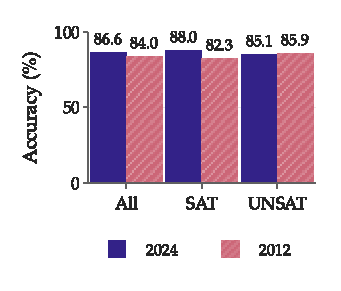
\includegraphics{figures/04/figs/sat_bar_2022.pdf}
        \caption{2022 SAT Competition}
        \label{fig:ch04:satpred22}
    \end{subfigure}\hfill
    \begin{subfigure}[b]{0.49\textwidth}
        \centering

        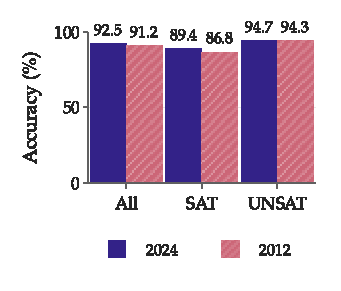
\includegraphics{figures/04/figs/sat_bar_2023.pdf}
        \caption{2023 SAT Competition}
        \label{fig:ch04:satpred23}
    \end{subfigure}
\end{figure*}

\subsection{Performance prediction}
The second downstream task we investigate is performance prediction, which has important applications in algorithm selection, configuration and benchmark generation. We refer to the methodology described in~\cite{HutEtAl14} and use a RF regressor as the EPM. It is important to note that for an accurate running time prediction we need to perform a $log_{10}$ transformation of running times prior to training the model, as done by Hutter
\emph{et al.}~\cite{HutEtAl14}. This transformation allows to capture the order of magnitude rather than small variations in the running time. The EPM then maps instance features to the log-transformed running times, and we aim to minimise the root mean squared error (RMSE) of the model, which is defined as $\sqrt{\frac{1}{n}\cdot \sum_{i=1}^n (\hat{y}_i-y_i)^2}$ for $n$ predicted running times  $\hat{y}_i$ and ground truth running times  $y_i$. Lower RMSE scores are better and 0 is the optimal value.
In line with the previous task, we perform inner and outer cross-validation and optimise the RF's hyperparameters for one hour using SMAC3.

We look into the performance of the EPM for running time prediction on all solvers from the 2022 and 2023 SAT Competitions. Here, we do not actually run solvers on instances to record their running times, but rather use the running times reported by the competitions. We display the results for the 10 best solvers from each competition in \cref{fig:ch04:rt_pred} (the results for all solvers can be found in the supplementary material). We see that using the features extracted by the new tool leads to the lower RMSE for all solvers, compared to using those extracted by the old tool. For some solvers, we observe a significantly lower RMSE, like Kissat{\_}MAB{\_}prop-no{\_}sym, where using the new tool decreases the RMSE from 0.84 to 0.69. \cref{fig:ch04:rmse_hists} shows the histogram of the error percentage for all solvers in the 2022 and 2023 SAT Competitions. We see that for the 2022 competition, the new tool has more instances with error rate lower than $10\%$ compared to the old version. For the 2023 competition, using the features extracted with the new version, more instances are predicted with less than $1\%$ error. Histograms per solver are available in \cref{sec:ch04:rts_hists_per_solver}.

\begin{figure*}[h]
    \caption[Running time prediction with old and new SATZilla features]{Root mean square error (RMSE) of (log-transformed) running time prediction using a random forest with features extracted by the old (SATZilla 2012; in rose) and the new tool (SATZilla 2024; in indigo), on SAT solvers from the 2022 and 2023 SAT Competitions. The new tool achieves lower RMSE for all solvers.}
    \label{fig:ch04:rt_pred}
    \begin{subfigure}[b]{0.99\textwidth}
        \centering

        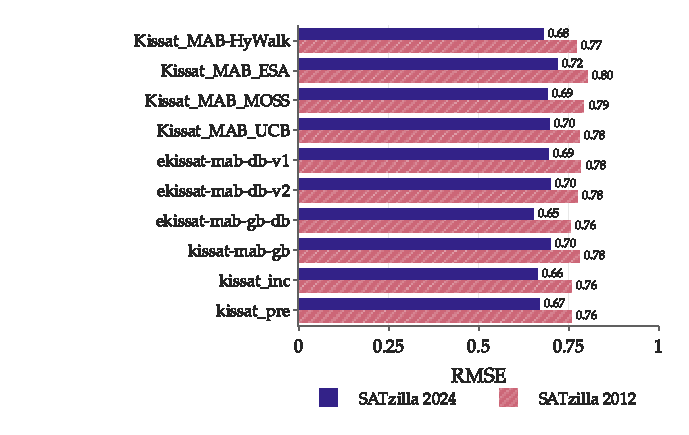
\includegraphics{figures/04/figs/rts_bar_2022.pdf}
        \caption{2022 SAT Competition}
        \label{fig:ch04:rt_pred22}
    \end{subfigure}\hfill
    \begin{subfigure}[b]{0.99\textwidth}
        \centering

        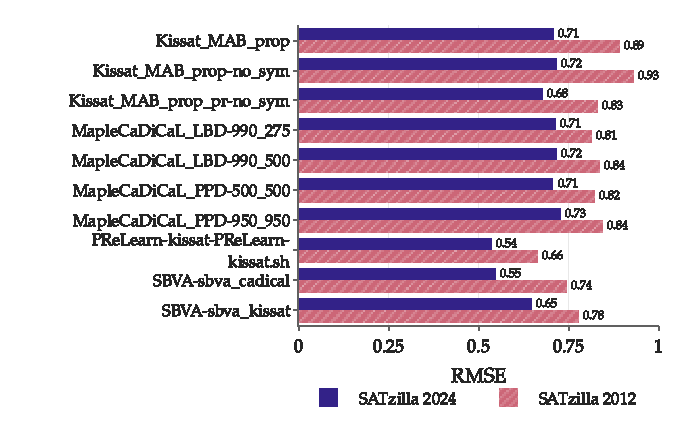
\includegraphics{figures/04/figs/rts_bar_2023.pdf}
        \caption{2023 SAT Competition}
        \label{fig:ch04:rt_pred23}
    \end{subfigure}
\end{figure*}

\begin{figure*}[h]
    \caption[Running time prediction error distributions]{Histogram of the error percentage of the root mean square error (RMSE) of (log-transformed) running time prediction using a random forest with features extracted by the old (SATZilla 2012; in rose) and the new tool (SATZilla 2024; in indigo), on SAT solvers from the 2022 and 2023 SAT Competitions. The new tool achieves lower error percentages.}
    \label{fig:ch04:rmse_hists}
    \begin{subfigure}[b]{0.49\textwidth}
        \centering

        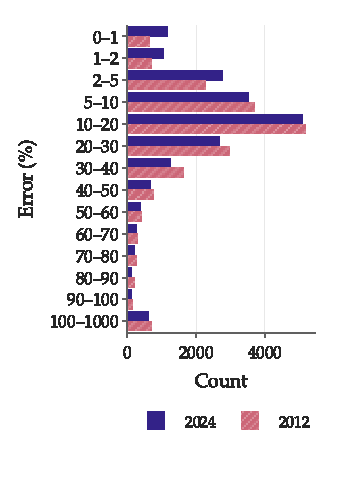
\includegraphics{figures/04/figs/acc_rt_pred_sc2022_both.pdf}
        \caption{2022 SAT Competition}
        \label{fig:ch04:rmse_hist_2022}
    \end{subfigure}\hfill
    \begin{subfigure}[b]{0.49\textwidth}
        \centering

        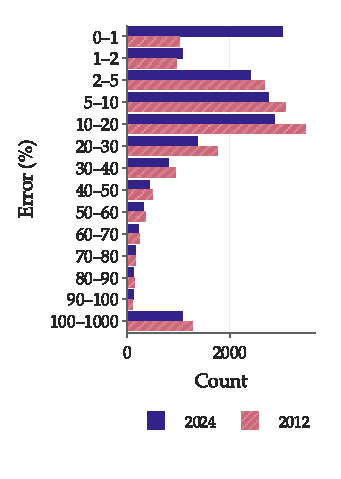
\includegraphics{figures/04/figs/acc_rt_pred_sc2023_both.pdf}
        \caption{2023 SAT Competition}
        \label{fig:ch04:rmse_hist_2023}
    \end{subfigure}
\end{figure*}

\subsection{Algorithm selection}
The third and final downstream task we consider is algorithm selection. In algorithm selection, given a set of instances $I$, a set of solvers (\emph{i.e.}, algorithm portfolio) $\mathbf{A}$ and a performance metric $m: \mathbf{A} \times I \rightarrow \mathbb{R}$, we build an algorithm selector $S: I \rightarrow \mathbf{A}$ such that its performance is optimal on the instance set $I$ according to the metric $m$.
We compare the performance of algorithm selection to two standard baselines, the single best solver (SBS; \emph{i.e}, the solver with the lowest overall running time) and the virtual best solver (VBS; \emph{i.e.}, the theoretical oracle which for each instance selects the actual best solver on it).

We measure the performance of algorithm selection using \textit{closed gap}, which is computed as $\frac{m_{SBS} - m_{S}}{m_{SBS} - m_{VBS}}$, (\emph{i.e.}, the closed gap stands for how much of the gap between the SBS and the VBS is closed by using the algorithm selector).
We then use AutoFolio~\cite{LinEtAl15} as an algorithm selector, which consists of multiple algorithm selection approaches, from which the best one is suggested by using algorithm configuration.
As algorithm portfolio for the selection, we use the 10 best solvers from each SAT competition. We train the selector for 8 hours.

\cref{fig:ch04:closed_gap} shows the closed gap results on the 2022 and 2023 SAT Competitions. Positive closed gap values on both scenarios using both the old and the new tool indicate that, in general, SATZilla features are useful for the algorithm selection task.
Importantly, features extracted with the new tool lead to better closed gap values on both scenarios.
In \cref{fig:ch04:ecdf_as}, we provide ECDF plots showing the fraction of instances solved over time. In the 2022 SAT Competition scenario, the old version of the tool performs worse than the SBS until a budget of approximately 1000 seconds, while the new version of the tool performs similarly to the SBS. After 1000 seconds, both versions of the SATZilla features perform similarly. In the 2023 SAT Competition scenario, the new tool performs better than the old one for budgets between 100 and 1000 seconds. With a budget of less than 10 seconds, the old tool solves more instances.
Overall, the ECDF plots reflect well what is shown in \cref{fig:ch04:closed_gap}, where we see that the new tool exhibits a few percents higher closed gap value.

\begin{figure}[h]
    \centering
    \caption[Algorithm selection closed gap with SATZilla features]{Closed gap values for the algorithm selection task using the old (SATZilla 2012; in rose) and the new tool (SATZilla 2024; in indigo) on the 2022 and 2023 SAT Competitions; higher is better.}
    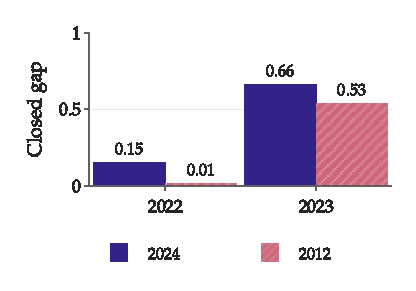
\includegraphics{figures/04/figs/as_bar_2023.pdf}
    \label{fig:ch04:closed_gap}
\end{figure}

\begin{figure*}[h]
    \caption[Algorithm selection ECDFs with SATZilla features]{ECDF plots for the algorithm selection task using the old (SATZilla 2012) and the new tool (SATZilla 2024) on the 2022 and 2023 SAT Competitions.}
    \label{fig:ch04:ecdf_as}
    \begin{subfigure}[b]{0.49\textwidth}
        \centering
        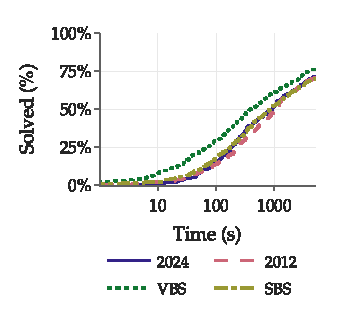
\includegraphics{figures/04/figs/ecds_af_2022.pdf}
        \caption{2022 SAT Competition}
        \label{fig:ch04:ecdf_as_2022}
    \end{subfigure}\hfill
    \begin{subfigure}[b]{0.49\textwidth}
        \centering
        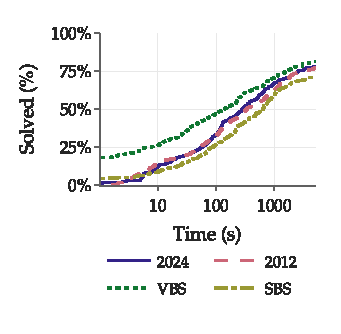
\includegraphics{figures/04/figs/ecds_af_2023.pdf}
        \caption{2023 SAT Competition}
        \label{fig:ch04:ecdf_as_2023}
    \end{subfigure}
\end{figure*}

\section{Conclusions}
\label{sec:ch04:conclusions}

In this chapter, we introduced an improved version of the well-known SATZilla feature extraction tool, motivated by the need to facilitate feature extraction through improved user infrastructure and bug fixes. Our new version combines updated preprocessing and probing solvers with more flexible time-limit handling. On the evaluated competition benchmarks, the combined update improves overall satisfiability prediction, lowers running time prediction error, and increases the closed gap for algorithm selection. As discussed in~\cref{sec:ch04:limitations}, these results concern the complete pipeline; they do not isolate the effects of preprocessing, feature availability, and individual probing solvers.

Our new SATZilla 2024 extraction tool aims to facilitate and promote the usage of SAT features even beyond their current scope. It is easily extensible and thus encourages building atop, \emph{e.g.}, by looking into features based on the recent developments in the explainability of SAT solvers \cite{ElfEtAl18}, or other advancements in SAT.

% \section{Running time prediction results}
% In this appendix, we present the full results of running time prediction for all solvers from the 2022 and 2023 SAT Competitions. In \cref{tab:ch04:full_rt_2022a,tab:ch04:full_rt_2022b} we show the results for the 2022 SAT Competition, where we see that our new tool constantly outperforms the old one. Similarly, in \cref{tab:ch04:full_rt_2023} we show the results for the 2023 SAT Competition, where using the features extracted by our new tool leads to lower RMSE than with the old one.
% \begin{table}[]
%     \centering
%     \caption[Running time prediction errors on SAT Competition 2022, part 1]{RMSE of random forest for predicting log-transformed running times of SAT solvers from the 2022 SAT Competition using the old and new SATZilla features.}
%     \label{tab:ch04:full_rt_2022a}
%     \begin{tabular}{c c c}
%         Solver & SATZilla 2012 & SATZilla 2024 \\
%         \hline
%         CaDiCaL-watchsat-lto & 0.70 & \textbf{0.63} \\
% CaDiCaL{\_}DVDL{\_}V1 & 0.73 & \textbf{0.65} \\
% CaDiCaL{\_}DVDL{\_}V2 & 0.75 & \textbf{0.65} \\
% CadicalReorder & 0.75 & \textbf{0.66} \\
% Cadical{\_}ESA & 0.75 & \textbf{0.66} \\
% IsaSAT & 0.73 & \textbf{0.64} \\
% Kissat-MAB-rephasing & 0.74 & \textbf{0.67} \\
% Kissat{\_}MAB-HyWalk & 0.77 & \textbf{0.68} \\
% Kissat{\_}MAB{\_}ESA & 0.80 & \textbf{0.72} \\
% Kissat{\_}MAB{\_}MOSS & 0.79 & \textbf{0.69} \\
% Kissat{\_}MAB{\_}UCB & 0.78 & \textbf{0.70} \\
% Kissat{\_}adaptive{\_}restart & 0.72 & \textbf{0.68} \\
% Kissat{\_}cfexp & 0.79 & \textbf{0.71} \\
% LSTech{\_}CaDiCaL & 0.77 & \textbf{0.63} \\
% LSTech{\_}Maple & 0.74 & \textbf{0.66} \\
% LSTech{\_}kissat & 0.76 & \textbf{0.67} \\
% LStech-Maple-BandSAT & 0.67 & \textbf{0.62} \\
% LStech-Maple-FPS & 0.74 & \textbf{0.65} \\
% LStech-Maple-HyWalk & 0.72 & \textbf{0.64} \\
% MapleLCMDistChrBt-DL-v3 & 0.61 & \textbf{0.58} \\
% MergeSat 4.0-rc-rc3 & 0.65 & \textbf{0.61} \\
% SLIME SC-2022 & 0.70 & \textbf{0.65} \\
% SLIME SC-2022-alpha & 0.70 & \textbf{0.66} \\
% SLIME SC-2022-beta & 0.71 & \textbf{0.66} \\
% SLIME SC-2022-gamma & 0.73 & \textbf{0.69} \\
% SeqFROST-ERE-All & 0.76 & \textbf{0.68} \\
% SeqFROST-NoExtend & 0.77 & \textbf{0.67} \\
% cadical-hack-gb & 0.73 & \textbf{0.62} \\
% cadical{\_}rel{\_}Scavel & 0.71 & \textbf{0.61} \\

%         \hline
%     \end{tabular}
% \end{table}

% \begin{table}[]
%     \centering
%     \caption[Running time prediction errors on SAT Competition 2022, part 2]{RMSE of random forest for predicting log-transformed running times of SAT solvers from the 2022 SAT Competition using the old and new SATZilla features (contd.).}
%     \label{tab:ch04:full_rt_2022b}
%     \begin{tabular}{c c c}
%         Solver & SATZilla 2012 & SATZilla 2024 \\
%         \hline
%         ekissat-mab-db-v1 & 0.78 & \textbf{0.69} \\
% ekissat-mab-db-v2 & 0.78 & \textbf{0.70} \\
% ekissat-mab-gb-db & 0.76 & \textbf{0.65} \\
% glucose-reboot & 0.78 & \textbf{0.68} \\
% hCaD{\_}V1-psids & 0.69 & \textbf{0.63} \\
% hCaD{\_}V2 & 0.68 & \textbf{0.64} \\
% hKis-psids & 0.69 & \textbf{0.59} \\
% hKis-sat & 0.79 & \textbf{0.69} \\
% hKis-unsat & 0.74 & \textbf{0.66} \\
% kissat-els-v1 & 0.76 & \textbf{0.67} \\
% kissat-els-v2 & 0.74 & \textbf{0.67} \\
% kissat-els-v3 & 0.78 & \textbf{0.67} \\
% kissat-els-v4 & 0.77 & \textbf{0.66} \\
% kissat-mab-gb & 0.78 & \textbf{0.70} \\
% kissat-sc2022-bulky & 0.76 & \textbf{0.69} \\
% kissat-sc2022-hyper & 0.76 & \textbf{0.70} \\
% kissat-sc2022-light & 0.75 & \textbf{0.69} \\
% kissat-watchsat-lto & 0.73 & \textbf{0.67} \\
% kissat{\_}inc & 0.76 & \textbf{0.66} \\
% kissat{\_}pre & 0.76 & \textbf{0.67} \\
% kissat{\_}relaxed & 0.72 & \textbf{0.67} \\
%         \hline
%     \end{tabular}
% \end{table}

% \begin{table}[]
%     \centering
%     \caption[Running time prediction errors on SAT Competition 2023]{RMSE of random forest for predicting log-transformed running times of SAT solvers from the 2023 SAT Competition using the old and new SATZilla features.}
%     \label{tab:ch04:full_rt_2023}
%     \begin{tabular}{c c c}
%         Solver & SATZilla 2012 & SATZilla 2024 \\
%         \hline
%         AMSAT{\_} & 0.80 & \textbf{0.77} \\
% BreakID-kissat-low.sh & 0.92 & \textbf{0.83} \\
% CaDiCaL{\_}vivinst & 0.84 & \textbf{0.73} \\
% Cadical{\_}ESA & 0.85 & \textbf{0.74} \\
% Cadical{\_}rel{\_}1.5.3.Scavel & 0.80 & \textbf{0.74} \\
% IsaSAT & 0.90 & \textbf{0.82} \\
% Kissat{\_}Inc{\_}ESA & 0.88 & \textbf{0.73} \\
% Kissat{\_}MAB{\_}Binary & 0.89 & \textbf{0.72} \\
% Kissat{\_}MAB{\_}Conflict & 0.87 & \textbf{0.72} \\
% Kissat{\_}MAB{\_}Conflict+ & 0.88 & \textbf{0.75} \\
% Kissat{\_}MAB{\_}DeepWalk+ & 0.87 & \textbf{0.73} \\
% Kissat{\_}MAB{\_}ESA & 0.91 & \textbf{0.74} \\
% Kissat{\_}MAB{\_}Rephases & 0.84 & \textbf{0.71} \\
% Kissat{\_}MAB{\_}prop & 0.89 & \textbf{0.71} \\
% Kissat{\_}MAB{\_}prop-no{\_}sym & 0.93 & \textbf{0.72} \\
% Kissat{\_}MAB{\_}prop{\_}pr-no{\_}sym & 0.83 & \textbf{0.68} \\
% MapleCaDiCaL{\_}LBD-990{\_}275 & 0.81 & \textbf{0.71} \\
% MapleCaDiCaL{\_}LBD-990{\_}500 & 0.84 & \textbf{0.72} \\
% MapleCaDiCaL{\_}PPD-500{\_}500 & 0.82 & \textbf{0.71} \\
% MapleCaDiCaL{\_}PPD-950{\_}950 & 0.84 & \textbf{0.73} \\
% MergeSat-bve{\_}gates & 0.75 & \textbf{0.71} \\
% MergeSat-bve{\_}semgates & 0.74 & \textbf{0.73} \\
% MergeSat-thread1 & 0.68 & \textbf{0.67} \\
% MiniSat+XorEngine & 0.79 & \textbf{0.77} \\
% PReLearn-kissat-PReLearn-kissat.sh & 0.66 & \textbf{0.54} \\
% PReLearn-kissat-PReLearn-tern-kissat.sh & 0.55 & \textbf{0.46} \\
% ReEncode-kissat-ReEncode-pair-kissat.sh & 0.75 & \textbf{0.68} \\
% SBVA-sbva{\_}cadical & 0.74 & \textbf{0.55} \\
% SBVA-sbva{\_}kissat & 0.78 & \textbf{0.65} \\
% SeqFROST & 0.81 & \textbf{0.73} \\
% SeqFROST-ERE-All & 0.81 & \textbf{0.71} \\
% SeqFROST-NoExtend & 0.79 & \textbf{0.74} \\
% hKis-psids & 0.81 & \textbf{0.72} \\
% hKis-sat{\_}psids & 0.80 & \textbf{0.79} \\
% hKis-unsat & 0.86 & \textbf{0.69} \\
% hKissatInc-unsat & 0.85 & \textbf{0.77} \\
% kissat-3.1.0 & 0.88 & \textbf{0.76} \\
% kissat-hywalk-exp & 0.85 & \textbf{0.70} \\
% kissat-hywalk-exp-gb & 0.89 & \textbf{0.74} \\
% kissat-hywalk-gb & 0.88 & \textbf{0.72} \\
% kissat{\_}incsp & 0.95 & \textbf{0.80} \\
% tabularasat-1.0.0 & 0.88 & \textbf{0.76} \\
%         \hline
%     \end{tabular}
% \end{table}

% \section{Running time prediction histograms}
% \label{sec:ch04:rts_hists_per_solver}
% We present the histograms for the RMSE values per solver for running time prediction in the figures in this section.
% \begin{figure}[p]
% \centering
% \caption[Per-solver prediction errors for SAT Competition 2022, part 1]{Per-solver running time prediction error percentages for SATZilla 2012 (rose, striped) and SATZilla 2024 (indigo).}
% \label{fig:ch04:rts_hists1}
% \begin{subfigure}[b]{0.49\textwidth}
%         \centering
%         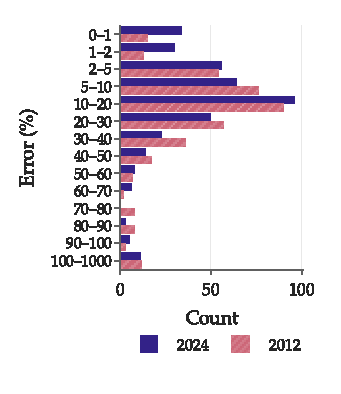
\includegraphics{figures/04/figs/acc_rt_pred_sc2022_both_CaDiCaL-watchsat-lto.pdf}
%         \caption{2022 Comp. CaDiCaL-watchsat-lto}
% \end{subfigure}\hfill
% \begin{subfigure}[b]{0.49\textwidth}
%         \centering
%         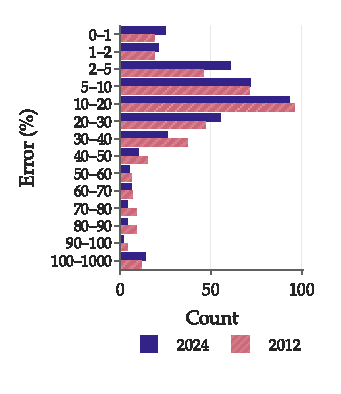
\includegraphics{figures/04/figs/acc_rt_pred_sc2022_both_CaDiCaL_DVDL_V1.pdf}
%         \caption{2022 Comp. CaDiCaL\_DVDL\_V1}
% \end{subfigure}
% \par\medskip
% \begin{subfigure}[b]{0.49\textwidth}
%         \centering
%         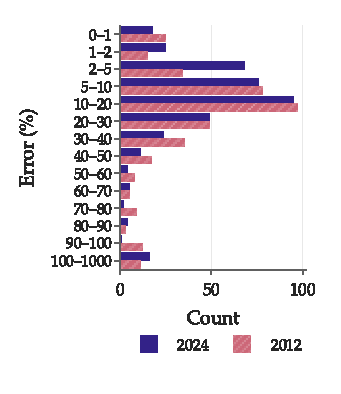
\includegraphics{figures/04/figs/acc_rt_pred_sc2022_both_CaDiCaL_DVDL_V2.pdf}
%         \caption{2022 Comp. CaDiCaL\_DVDL\_V2}
% \end{subfigure}\hfill
% \begin{subfigure}[b]{0.49\textwidth}
%         \centering
%         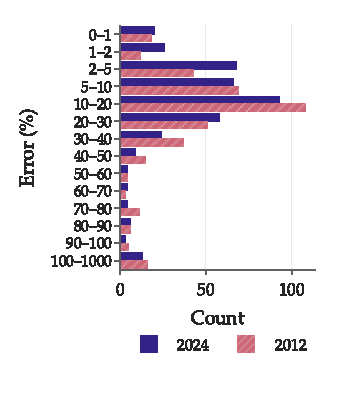
\includegraphics{figures/04/figs/acc_rt_pred_sc2022_both_CadicalReorder.pdf}
%         \caption{2022 Comp. CadicalReorder}
% \end{subfigure}
% \end{figure}
% \begin{figure}[p]
% \centering
% \caption[Per-solver prediction errors for SAT Competition 2022, part 2]{Per-solver running time prediction error percentages for SATZilla 2012 (rose, striped) and SATZilla 2024 (indigo).}
% \label{fig:ch04:rts_hists1b}
% \begin{subfigure}[b]{0.49\textwidth}
%         \centering
%         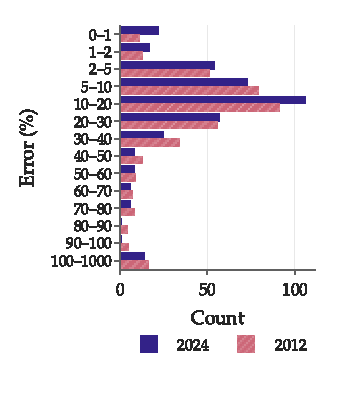
\includegraphics{figures/04/figs/acc_rt_pred_sc2022_both_Cadical_ESA.pdf}
%         \caption{2022 Comp. Cadical\_ESA}
% \end{subfigure}\hfill
% \begin{subfigure}[b]{0.49\textwidth}
%         \centering
%         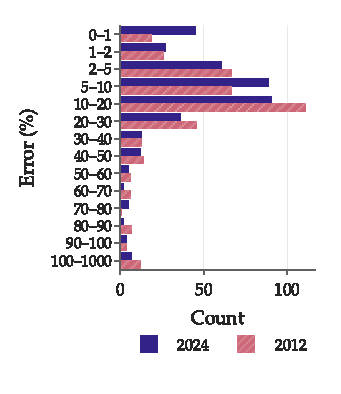
\includegraphics{figures/04/figs/acc_rt_pred_sc2022_both_IsaSAT.pdf}
%         \caption{2022 Comp. IsaSAT}
% \end{subfigure}
% \par\medskip
% \begin{subfigure}[b]{0.49\textwidth}
%         \centering
%         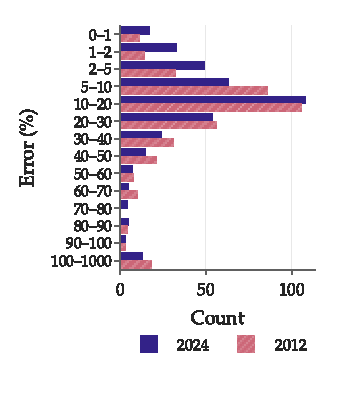
\includegraphics{figures/04/figs/acc_rt_pred_sc2022_both_Kissat-MAB-rephasing.pdf}
%         \caption{2022 Comp. Kissat-MAB-rephasing}
% \end{subfigure}\hfill
% \begin{subfigure}[b]{0.49\textwidth}
%         \centering
%         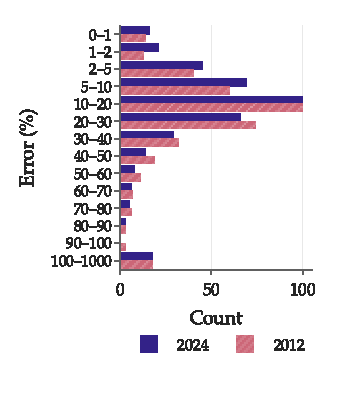
\includegraphics{figures/04/figs/acc_rt_pred_sc2022_both_Kissat_MAB-HyWalk.pdf}
%         \caption{2022 Comp. Kissat\_MAB-HyWalk}
% \end{subfigure}
% \end{figure}
% \begin{figure}[p]
% \centering
% \caption[Per-solver prediction errors for SAT Competition 2022, part 3]{Per-solver running time prediction error percentages for SATZilla 2012 (rose, striped) and SATZilla 2024 (indigo).}
% \label{fig:ch04:rts_hists2}
% \begin{subfigure}[b]{0.49\textwidth}
%         \centering
%         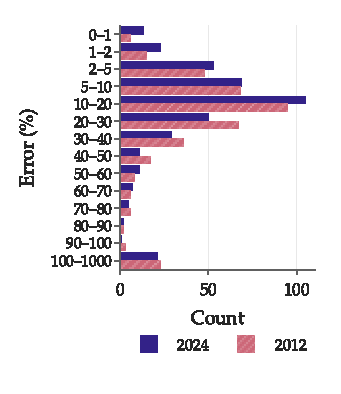
\includegraphics{figures/04/figs/acc_rt_pred_sc2022_both_Kissat_MAB_ESA.pdf}
%         \caption{2022 Comp. Kissat\_MAB\_ESA}
% \end{subfigure}\hfill
% \begin{subfigure}[b]{0.49\textwidth}
%         \centering
%         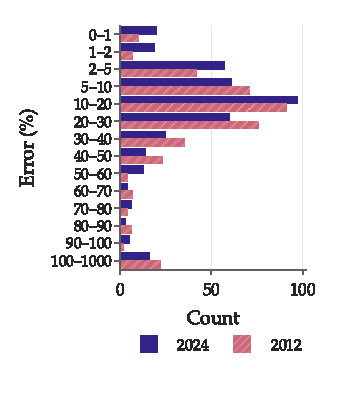
\includegraphics{figures/04/figs/acc_rt_pred_sc2022_both_Kissat_MAB_MOSS.pdf}
%         \caption{2022 Comp. Kissat\_MAB\_MOSS}
% \end{subfigure}
% \par\medskip
% \begin{subfigure}[b]{0.49\textwidth}
%         \centering
%         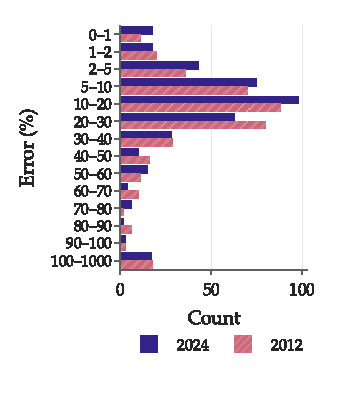
\includegraphics{figures/04/figs/acc_rt_pred_sc2022_both_Kissat_MAB_UCB.pdf}
%         \caption{2022 Comp. Kissat\_MAB\_UCB}
% \end{subfigure}\hfill
% \begin{subfigure}[b]{0.49\textwidth}
%         \centering
%         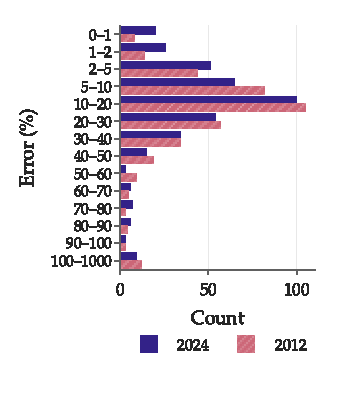
\includegraphics{figures/04/figs/acc_rt_pred_sc2022_both_Kissat_adaptive_restart.pdf}
%         \caption{2022 Comp. Kissat\_adaptive\_restart}
% \end{subfigure}
% \end{figure}
% \begin{figure}[p]
% \centering
% \caption[Per-solver prediction errors for SAT Competition 2022, part 4]{Per-solver running time prediction error percentages for SATZilla 2012 (rose, striped) and SATZilla 2024 (indigo).}
% \label{fig:ch04:rts_hists2b}
% \begin{subfigure}[b]{0.49\textwidth}
%         \centering
%         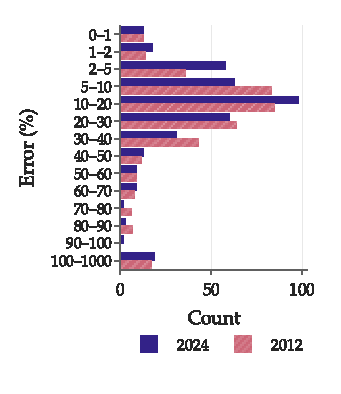
\includegraphics{figures/04/figs/acc_rt_pred_sc2022_both_Kissat_cfexp.pdf}
%         \caption{2022 Comp. Kissat\_cfexp}
% \end{subfigure}\hfill
% \begin{subfigure}[b]{0.49\textwidth}
%         \centering
%         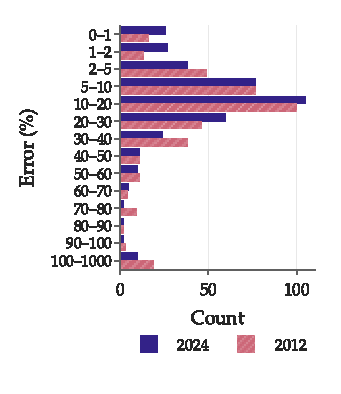
\includegraphics{figures/04/figs/acc_rt_pred_sc2022_both_LSTech_CaDiCaL.pdf}
%         \caption{2022 Comp. LSTech\_CaDiCaL}
% \end{subfigure}
% \par\medskip
% \begin{subfigure}[b]{0.49\textwidth}
%         \centering
%         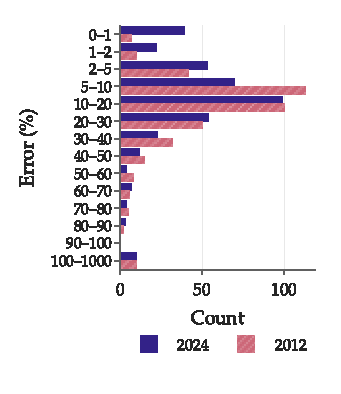
\includegraphics{figures/04/figs/acc_rt_pred_sc2022_both_LSTech_Maple.pdf}
%         \caption{2022 Comp. LSTech\_Maple}
% \end{subfigure}\hfill
% \begin{subfigure}[b]{0.49\textwidth}
%         \centering
%         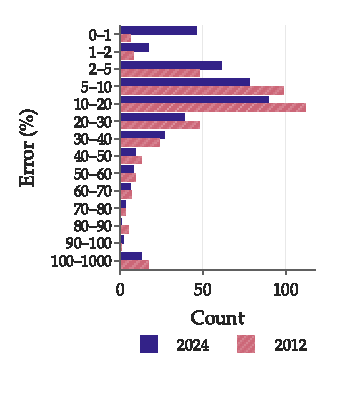
\includegraphics{figures/04/figs/acc_rt_pred_sc2022_both_LSTech_kissat.pdf}
%         \caption{2022 Comp. LSTech\_kissat}
% \end{subfigure}
% \end{figure}
% \begin{figure}[p]
% \centering
% \caption[Per-solver prediction errors for SAT Competition 2022, part 5]{Per-solver running time prediction error percentages for SATZilla 2012 (rose, striped) and SATZilla 2024 (indigo).}
% \label{fig:ch04:rts_hists3}
% \begin{subfigure}[b]{0.49\textwidth}
%         \centering
%         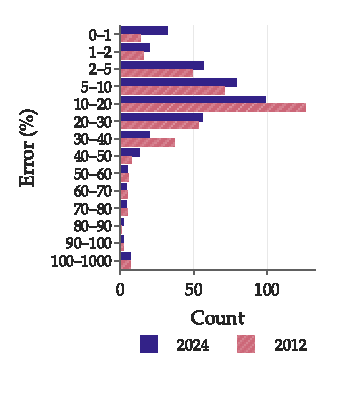
\includegraphics{figures/04/figs/acc_rt_pred_sc2022_both_LStech-Maple-BandSAT.pdf}
%         \caption{2022 Comp. LStech-Maple-BandSAT}
% \end{subfigure}\hfill
% \begin{subfigure}[b]{0.49\textwidth}
%         \centering
%         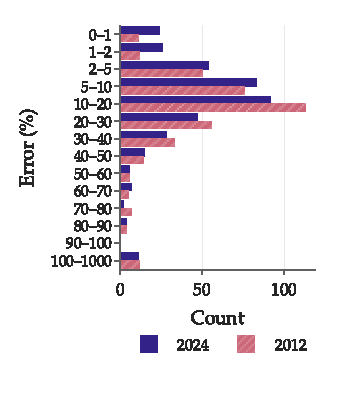
\includegraphics{figures/04/figs/acc_rt_pred_sc2022_both_LStech-Maple-FPS.pdf}
%         \caption{2022 Comp. LStech-Maple-FPS}
% \end{subfigure}
% \par\medskip
% \begin{subfigure}[b]{0.49\textwidth}
%         \centering
%         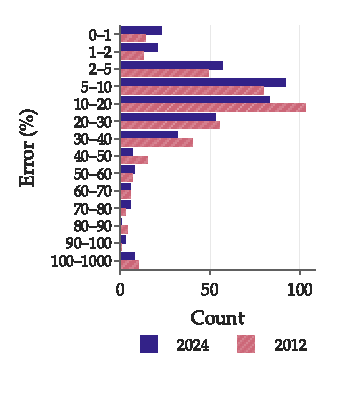
\includegraphics{figures/04/figs/acc_rt_pred_sc2022_both_LStech-Maple-HyWalk.pdf}
%         \caption{2022 Comp. LStech-Maple-HyWalk}
% \end{subfigure}\hfill
% \begin{subfigure}[b]{0.49\textwidth}
%         \centering
%         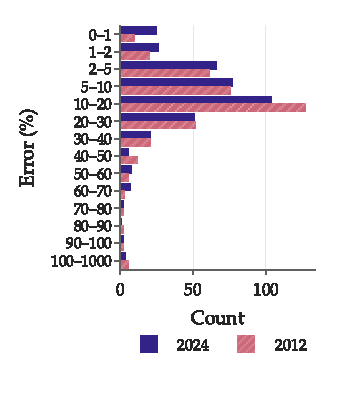
\includegraphics{figures/04/figs/acc_rt_pred_sc2022_both_MapleLCMDistChrBt-DL-v3.pdf}
%         \caption{2022 Comp. MapleLCMDistChrBt-DL-v3}
% \end{subfigure}
% \end{figure}
% \begin{figure}[p]
% \centering
% \caption[Per-solver prediction errors for SAT Competition 2022, part 6]{Per-solver running time prediction error percentages for SATZilla 2012 (rose, striped) and SATZilla 2024 (indigo).}
% \label{fig:ch04:rts_hists3b}
% \begin{subfigure}[b]{0.49\textwidth}
%         \centering
%         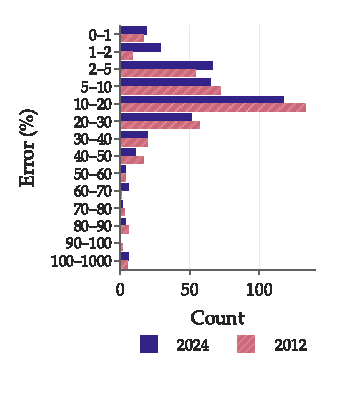
\includegraphics{figures/04/figs/acc_rt_pred_sc2022_both_MergeSat 4.0-rc-rc3.pdf}
%         \caption{2022 Comp. MergeSat 4.0-rc-rc3}
% \end{subfigure}\hfill
% \begin{subfigure}[b]{0.49\textwidth}
%         \centering
%         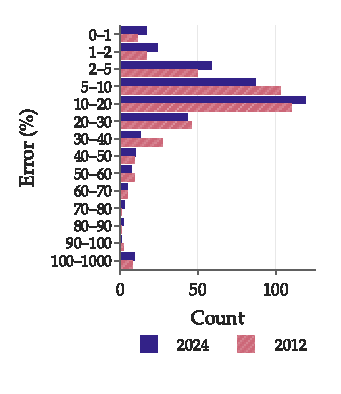
\includegraphics{figures/04/figs/acc_rt_pred_sc2022_both_SLIME SC-2022.pdf}
%         \caption{2022 Comp. SLIME SC-2022}
% \end{subfigure}
% \par\medskip
% \begin{subfigure}[b]{0.49\textwidth}
%         \centering
%         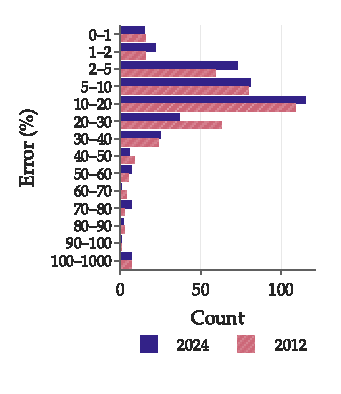
\includegraphics{figures/04/figs/acc_rt_pred_sc2022_both_SLIME SC-2022-alpha.pdf}
%         \caption{2022 Comp. SLIME SC-2022-alpha}
% \end{subfigure}\hfill
% \begin{subfigure}[b]{0.49\textwidth}
%         \centering
%         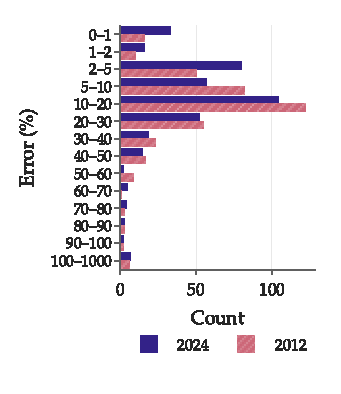
\includegraphics{figures/04/figs/acc_rt_pred_sc2022_both_SLIME SC-2022-beta.pdf}
%         \caption{2022 Comp. SLIME SC-2022-beta}
% \end{subfigure}
% \end{figure}
% \begin{figure}[p]
% \centering
% \caption[Per-solver prediction errors for SAT Competition 2022, part 7]{Per-solver running time prediction error percentages for SATZilla 2012 (rose, striped) and SATZilla 2024 (indigo).}
% \label{fig:ch04:rts_hists4}
% \begin{subfigure}[b]{0.49\textwidth}
%         \centering
%         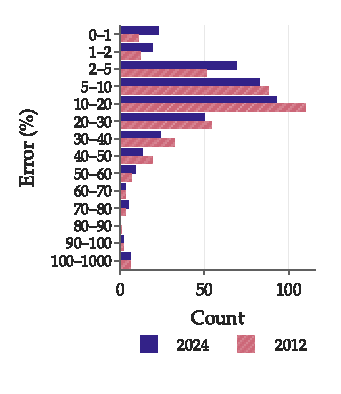
\includegraphics{figures/04/figs/acc_rt_pred_sc2022_both_SLIME SC-2022-gamma.pdf}
%         \caption{2022 Comp. SLIME SC-2022-gamma}
% \end{subfigure}\hfill
% \begin{subfigure}[b]{0.49\textwidth}
%         \centering
%         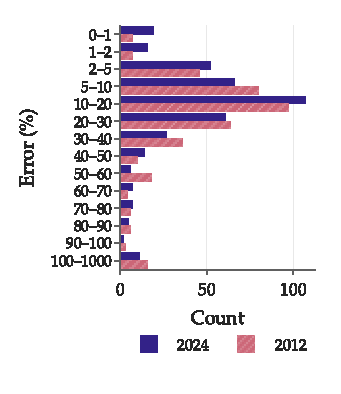
\includegraphics{figures/04/figs/acc_rt_pred_sc2022_both_SeqFROST-ERE-All.pdf}
%         \caption{2022 Comp. SeqFROST-ERE-All}
% \end{subfigure}
% \par\medskip
% \begin{subfigure}[b]{0.49\textwidth}
%         \centering
%         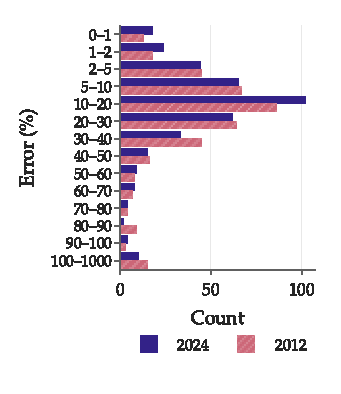
\includegraphics{figures/04/figs/acc_rt_pred_sc2022_both_SeqFROST-NoExtend.pdf}
%         \caption{2022 Comp. SeqFROST-NoExtend}
% \end{subfigure}\hfill
% \begin{subfigure}[b]{0.49\textwidth}
%         \centering
%         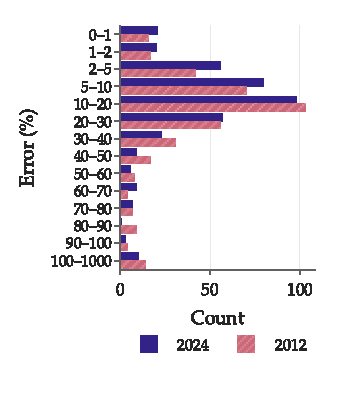
\includegraphics{figures/04/figs/acc_rt_pred_sc2022_both_cadical-hack-gb.pdf}
%         \caption{2022 Comp. cadical-hack-gb}
% \end{subfigure}
% \end{figure}
% \begin{figure}[p]
% \centering
% \caption[Per-solver prediction errors for SAT Competition 2022, part 8]{Per-solver running time prediction error percentages for SATZilla 2012 (rose, striped) and SATZilla 2024 (indigo).}
% \label{fig:ch04:rts_hists4b}
% \begin{subfigure}[b]{0.49\textwidth}
%         \centering
%         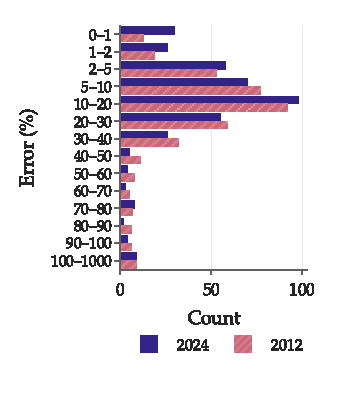
\includegraphics{figures/04/figs/acc_rt_pred_sc2022_both_cadical_rel_Scavel.pdf}
%         \caption{2022 Comp. cadical\_rel\_Scavel}
% \end{subfigure}\hfill
% \begin{subfigure}[b]{0.49\textwidth}
%         \centering
%         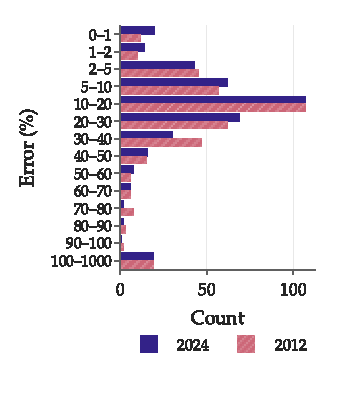
\includegraphics{figures/04/figs/acc_rt_pred_sc2022_both_ekissat-mab-db-v1.pdf}
%         \caption{2022 Comp. ekissat-mab-db-v1}
% \end{subfigure}
% \par\medskip
% \begin{subfigure}[b]{0.49\textwidth}
%         \centering
%         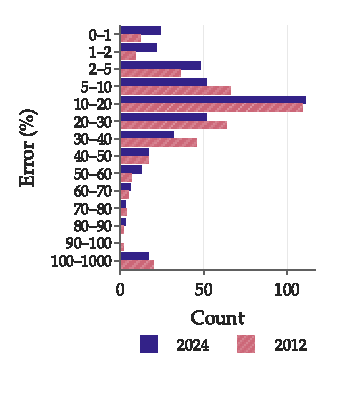
\includegraphics{figures/04/figs/acc_rt_pred_sc2022_both_ekissat-mab-db-v2.pdf}
%         \caption{2022 Comp. ekissat-mab-db-v2}
% \end{subfigure}\hfill
% \begin{subfigure}[b]{0.49\textwidth}
%         \centering
%         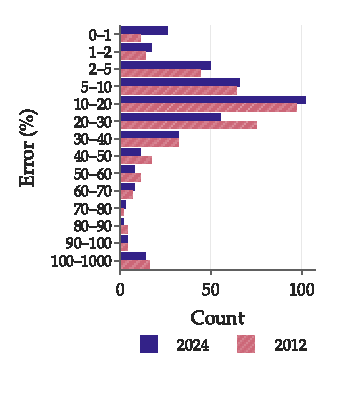
\includegraphics{figures/04/figs/acc_rt_pred_sc2022_both_ekissat-mab-gb-db.pdf}
%         \caption{2022 Comp. ekissat-mab-gb-db}
% \end{subfigure}
% \end{figure}
% \begin{figure}[p]
% \centering
% \caption[Per-solver prediction errors for SAT Competition 2022, part 9]{Per-solver running time prediction error percentages for SATZilla 2012 (rose, striped) and SATZilla 2024 (indigo).}
% \label{fig:ch04:rts_hists5}
% \begin{subfigure}[b]{0.49\textwidth}
%         \centering
%         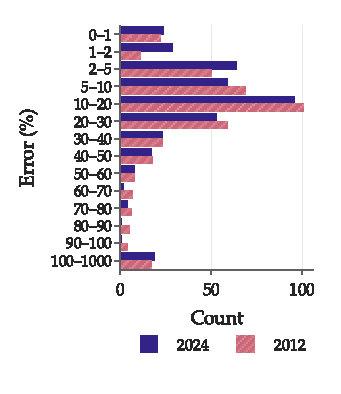
\includegraphics{figures/04/figs/acc_rt_pred_sc2022_both_glucose-reboot.pdf}
%         \caption{2022 Comp. glucose-reboot}
% \end{subfigure}\hfill
% \begin{subfigure}[b]{0.49\textwidth}
%         \centering
%         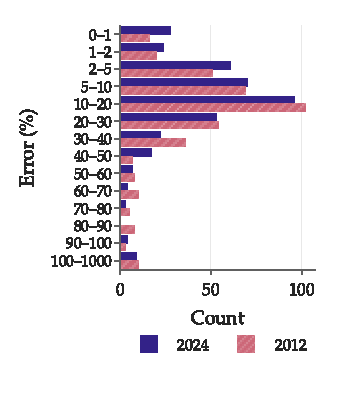
\includegraphics{figures/04/figs/acc_rt_pred_sc2022_both_hCaD_V1-psids.pdf}
%         \caption{2022 Comp. hCaD\_V1-psids}
% \end{subfigure}
% \par\medskip
% \begin{subfigure}[b]{0.49\textwidth}
%         \centering
%         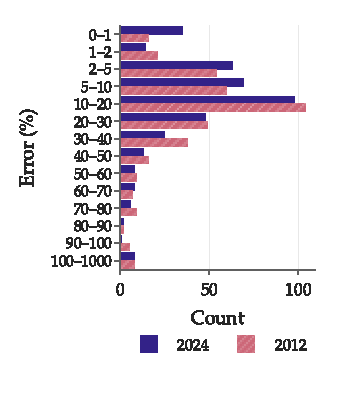
\includegraphics{figures/04/figs/acc_rt_pred_sc2022_both_hCaD_V2.pdf}
%         \caption{2022 Comp. hCaD\_V2}
% \end{subfigure}\hfill
% \begin{subfigure}[b]{0.49\textwidth}
%         \centering
%         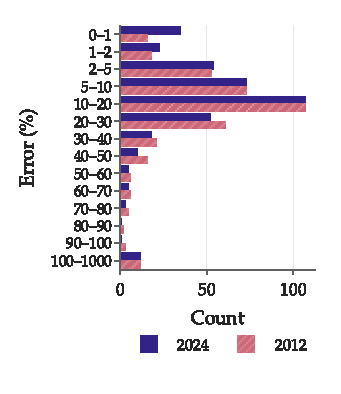
\includegraphics{figures/04/figs/acc_rt_pred_sc2022_both_hKis-psids.pdf}
%         \caption{2022 Comp. hKis-psids}
% \end{subfigure}
% \end{figure}
% \begin{figure}[p]
% \centering
% \caption[Per-solver prediction errors for SAT Competition 2022, part 10]{Per-solver running time prediction error percentages for SATZilla 2012 (rose, striped) and SATZilla 2024 (indigo).}
% \label{fig:ch04:rts_hists5b}
% \begin{subfigure}[b]{0.49\textwidth}
%         \centering
%         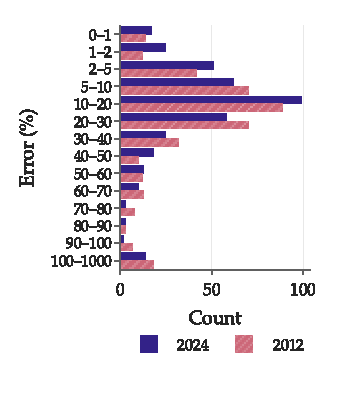
\includegraphics{figures/04/figs/acc_rt_pred_sc2022_both_hKis-sat.pdf}
%         \caption{2022 Comp. hKis-sat}
% \end{subfigure}\hfill
% \begin{subfigure}[b]{0.49\textwidth}
%         \centering
%         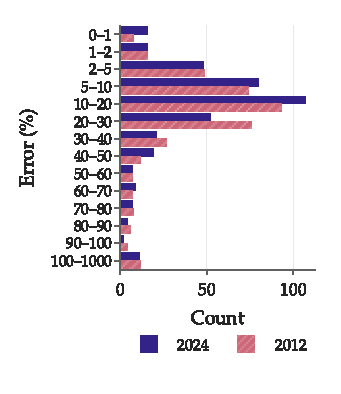
\includegraphics{figures/04/figs/acc_rt_pred_sc2022_both_hKis-unsat.pdf}
%         \caption{2022 Comp. hKis-unsat}
% \end{subfigure}
% \par\medskip
% \begin{subfigure}[b]{0.49\textwidth}
%         \centering
%         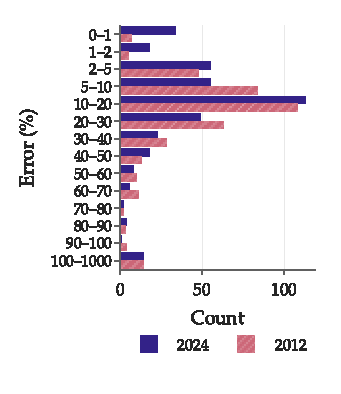
\includegraphics{figures/04/figs/acc_rt_pred_sc2022_both_kissat-els-v1.pdf}
%         \caption{2022 Comp. kissat-els-v1}
% \end{subfigure}\hfill
% \begin{subfigure}[b]{0.49\textwidth}
%         \centering
%         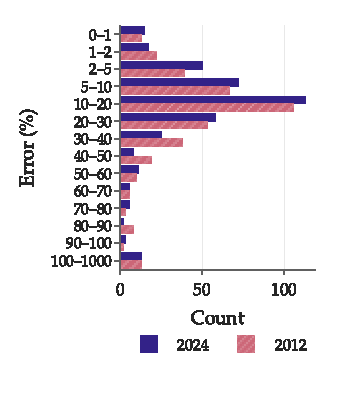
\includegraphics{figures/04/figs/acc_rt_pred_sc2022_both_kissat-els-v2.pdf}
%         \caption{2022 Comp. kissat-els-v2}
% \end{subfigure}
% \end{figure}
% \begin{figure}[p]
% \centering
% \caption[Per-solver prediction errors for SAT Competition 2022, part 11]{Per-solver running time prediction error percentages for SATZilla 2012 (rose, striped) and SATZilla 2024 (indigo).}
% \label{fig:ch04:rts_hists6}
% \begin{subfigure}[b]{0.49\textwidth}
%         \centering
%         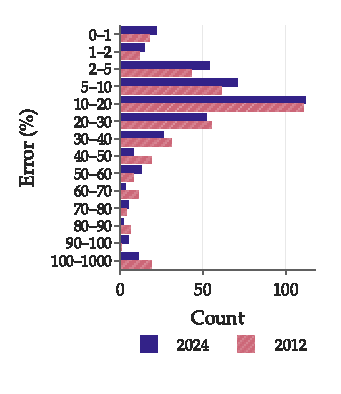
\includegraphics{figures/04/figs/acc_rt_pred_sc2022_both_kissat-els-v3.pdf}
%         \caption{2022 Comp. kissat-els-v3}
% \end{subfigure}\hfill
% \begin{subfigure}[b]{0.49\textwidth}
%         \centering
%         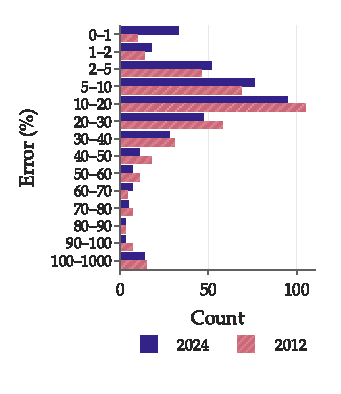
\includegraphics{figures/04/figs/acc_rt_pred_sc2022_both_kissat-els-v4.pdf}
%         \caption{2022 Comp. kissat-els-v4}
% \end{subfigure}
% \par\medskip
% \begin{subfigure}[b]{0.49\textwidth}
%         \centering
%         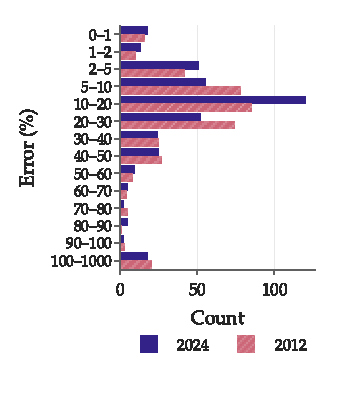
\includegraphics{figures/04/figs/acc_rt_pred_sc2022_both_kissat-mab-gb.pdf}
%         \caption{2022 Comp. kissat-mab-gb}
% \end{subfigure}\hfill
% \begin{subfigure}[b]{0.49\textwidth}
%         \centering
%         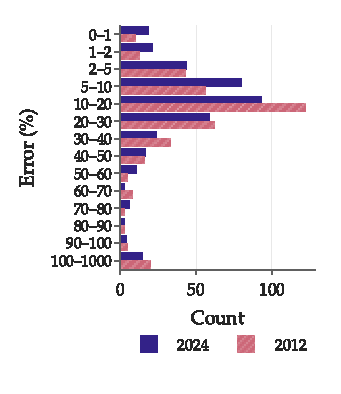
\includegraphics{figures/04/figs/acc_rt_pred_sc2022_both_kissat-sc2022-bulky.pdf}
%         \caption{2022 Comp. kissat-sc2022-bulky}
% \end{subfigure}
% \end{figure}
% \begin{figure}[p]
% \centering
% \caption[Per-solver prediction errors for SAT Competition 2022, part 12]{Per-solver running time prediction error percentages for SATZilla 2012 (rose, striped) and SATZilla 2024 (indigo).}
% \label{fig:ch04:rts_hists6b}
% \begin{subfigure}[b]{0.49\textwidth}
%         \centering
%         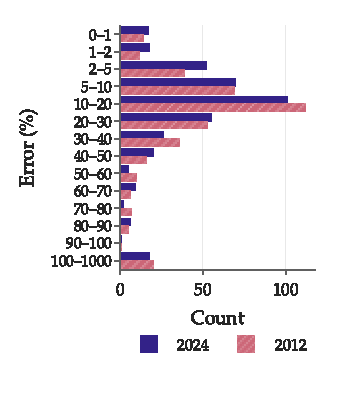
\includegraphics{figures/04/figs/acc_rt_pred_sc2022_both_kissat-sc2022-hyper.pdf}
%         \caption{2022 Comp. kissat-sc2022-hyper}
% \end{subfigure}\hfill
% \begin{subfigure}[b]{0.49\textwidth}
%         \centering
%         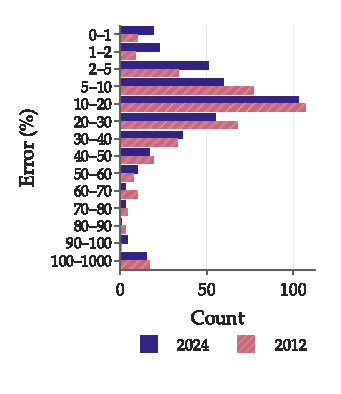
\includegraphics{figures/04/figs/acc_rt_pred_sc2022_both_kissat-sc2022-light.pdf}
%         \caption{2022 Comp. kissat-sc2022-light}
% \end{subfigure}
% \par\medskip
% \begin{subfigure}[b]{0.49\textwidth}
%         \centering
%         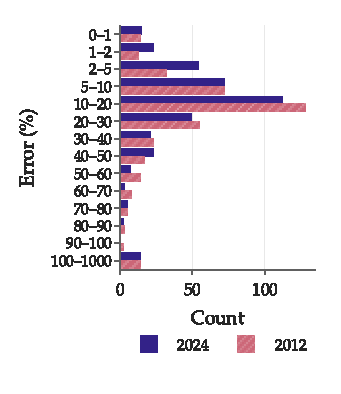
\includegraphics{figures/04/figs/acc_rt_pred_sc2022_both_kissat-watchsat-lto.pdf}
%         \caption{2022 Comp. kissat-watchsat-lto}
% \end{subfigure}\hfill
% \begin{subfigure}[b]{0.49\textwidth}
%         \centering
%         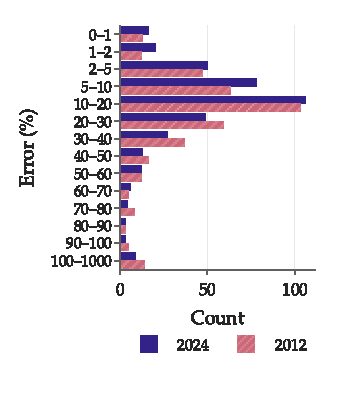
\includegraphics{figures/04/figs/acc_rt_pred_sc2022_both_kissat_inc.pdf}
%         \caption{2022 Comp. kissat\_inc}
% \end{subfigure}
% \end{figure}
% \begin{figure}[p]
% \centering
% \caption[Per-solver prediction errors for SAT Competition 2022, part 13]{Per-solver running time prediction error percentages for SATZilla 2012 (rose, striped) and SATZilla 2024 (indigo).}
% \label{fig:ch04:rts_hists7}
% \begin{subfigure}[b]{0.49\textwidth}
%         \centering
%         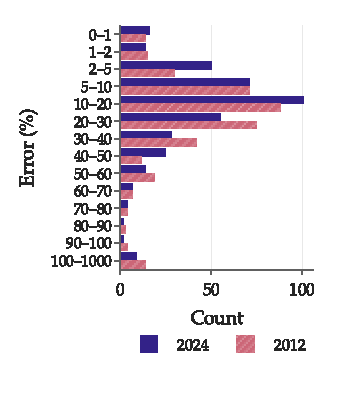
\includegraphics{figures/04/figs/acc_rt_pred_sc2022_both_kissat_pre.pdf}
%         \caption{2022 Comp. kissat\_pre}
% \end{subfigure}\hfill
% \begin{subfigure}[b]{0.49\textwidth}
%         \centering
%         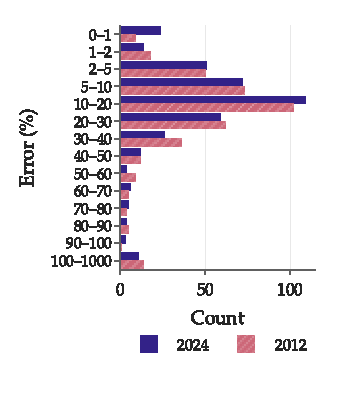
\includegraphics{figures/04/figs/acc_rt_pred_sc2022_both_kissat_relaxed.pdf}
%         \caption{2022 Comp. kissat\_relaxed}
% \end{subfigure}
% \par\medskip
% \begin{subfigure}[b]{0.49\textwidth}
%         \centering
%         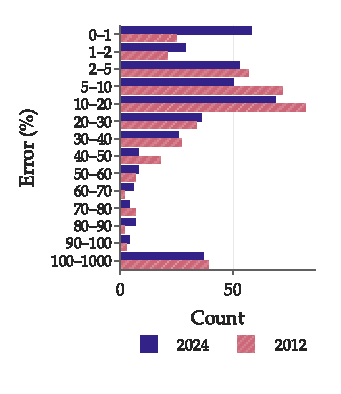
\includegraphics{figures/04/figs/acc_rt_pred_sc2023_both_AMSAT_.pdf}
%         \caption{2023 Comp. AMSAT\_}
% \end{subfigure}\hfill
% \begin{subfigure}[b]{0.49\textwidth}
%         \centering
%         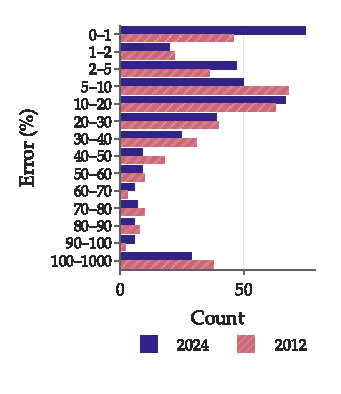
\includegraphics{figures/04/figs/acc_rt_pred_sc2023_both_BreakID-kissat-low.sh.pdf}
%         \caption{2023 Comp. BreakID-kissat-low.sh}
% \end{subfigure}
% \end{figure}
% \begin{figure}[p]
% \centering
% \caption[Per-solver prediction errors for SAT Competition 2023, part 2]{Per-solver running time prediction error percentages for SATZilla 2012 (rose, striped) and SATZilla 2024 (indigo).}
% \label{fig:ch04:rts_hists7b}
% \begin{subfigure}[b]{0.49\textwidth}
%         \centering
%         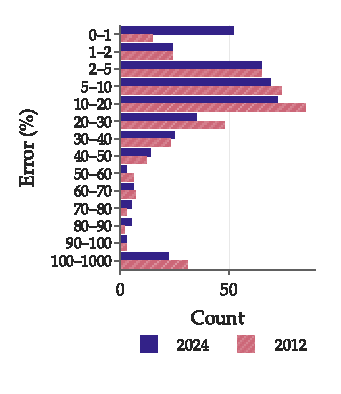
\includegraphics{figures/04/figs/acc_rt_pred_sc2023_both_CaDiCaL_vivinst.pdf}
%         \caption{2023 Comp. CaDiCaL\_vivinst}
% \end{subfigure}\hfill
% \begin{subfigure}[b]{0.49\textwidth}
%         \centering
%         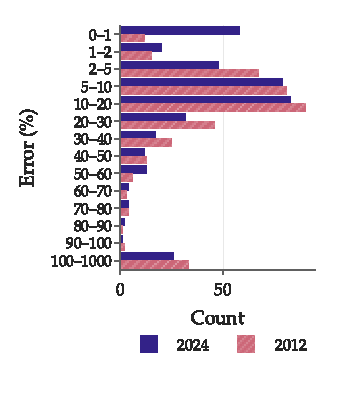
\includegraphics{figures/04/figs/acc_rt_pred_sc2023_both_Cadical_ESA.pdf}
%         \caption{2023 Comp. Cadical\_ESA}
% \end{subfigure}
% \par\medskip
% \begin{subfigure}[b]{0.49\textwidth}
%         \centering
%         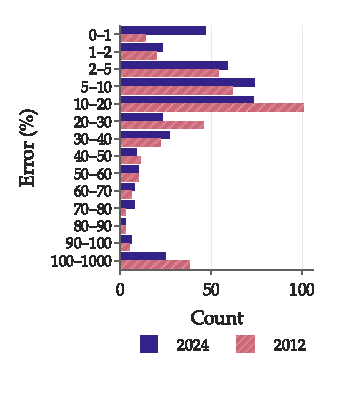
\includegraphics{figures/04/figs/acc_rt_pred_sc2023_both_Cadical_rel_1.5.3.Scavel.pdf}
%         \caption{2023 Comp. Cadical\_rel\_1.5.3.Scavel}
% \end{subfigure}\hfill
% \begin{subfigure}[b]{0.49\textwidth}
%         \centering
%         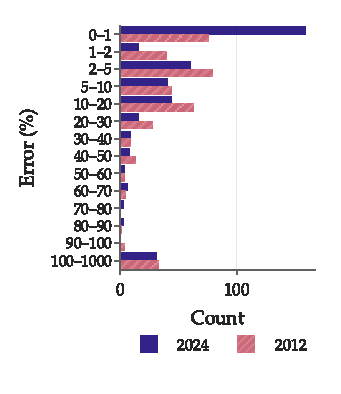
\includegraphics{figures/04/figs/acc_rt_pred_sc2023_both_IsaSAT.pdf}
%         \caption{2023 Comp. IsaSAT}
% \end{subfigure}
% \end{figure}
% \begin{figure}[p]
% \centering
% \caption[Per-solver prediction errors for SAT Competition 2023, part 3]{Per-solver running time prediction error percentages for SATZilla 2012 (rose, striped) and SATZilla 2024 (indigo).}
% \label{fig:ch04:rts_hists8}
% \begin{subfigure}[b]{0.49\textwidth}
%         \centering
%         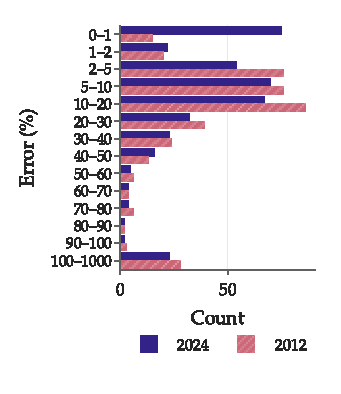
\includegraphics{figures/04/figs/acc_rt_pred_sc2023_both_Kissat_Inc_ESA.pdf}
%         \caption{2023 Comp. Kissat\_Inc\_ESA}
% \end{subfigure}\hfill
% \begin{subfigure}[b]{0.49\textwidth}
%         \centering
%         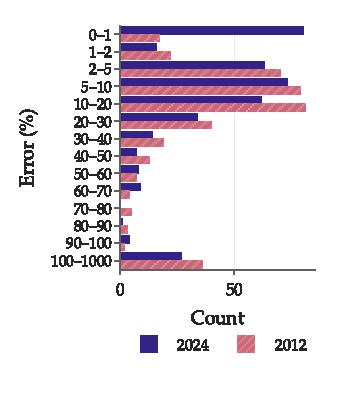
\includegraphics{figures/04/figs/acc_rt_pred_sc2023_both_Kissat_MAB_Binary.pdf}
%         \caption{2023 Comp. Kissat\_MAB\_Binary}
% \end{subfigure}
% \par\medskip
% \begin{subfigure}[b]{0.49\textwidth}
%         \centering
%         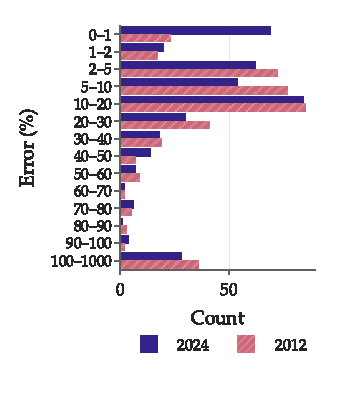
\includegraphics{figures/04/figs/acc_rt_pred_sc2023_both_Kissat_MAB_Conflict.pdf}
%         \caption{2023 Comp. Kissat\_MAB\_Conflict}
% \end{subfigure}\hfill
% \begin{subfigure}[b]{0.49\textwidth}
%         \centering
%         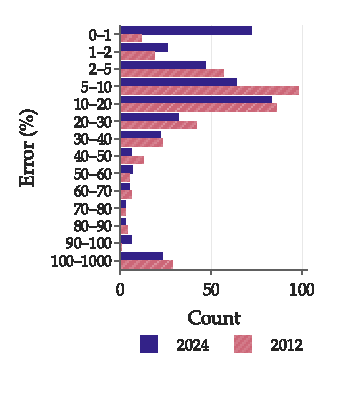
\includegraphics{figures/04/figs/acc_rt_pred_sc2023_both_Kissat_MAB_Conflict+.pdf}
%         \caption{2023 Comp. Kissat\_MAB\_Conflict+}
% \end{subfigure}
% \end{figure}
% \begin{figure}[p]
% \centering
% \caption[Per-solver prediction errors for SAT Competition 2023, part 4]{Per-solver running time prediction error percentages for SATZilla 2012 (rose, striped) and SATZilla 2024 (indigo).}
% \label{fig:ch04:rts_hists8b}
% \begin{subfigure}[b]{0.49\textwidth}
%         \centering
%         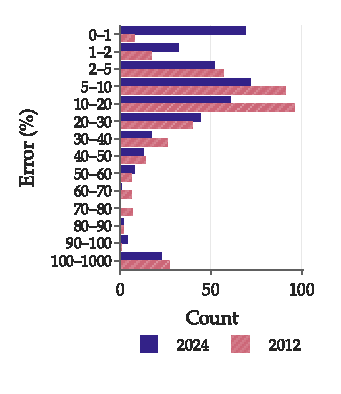
\includegraphics{figures/04/figs/acc_rt_pred_sc2023_both_Kissat_MAB_DeepWalk+.pdf}
%         \caption{2023 Comp. Kissat\_MAB\_DeepWalk+}
% \end{subfigure}\hfill
% \begin{subfigure}[b]{0.49\textwidth}
%         \centering
%         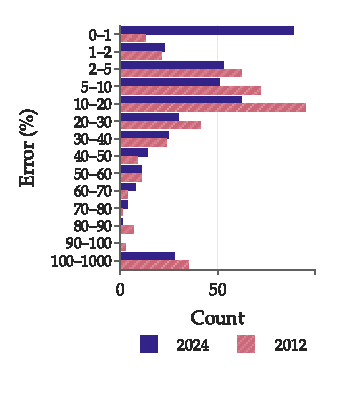
\includegraphics{figures/04/figs/acc_rt_pred_sc2023_both_Kissat_MAB_ESA.pdf}
%         \caption{2023 Comp. Kissat\_MAB\_ESA}
% \end{subfigure}
% \par\medskip
% \begin{subfigure}[b]{0.49\textwidth}
%         \centering
%         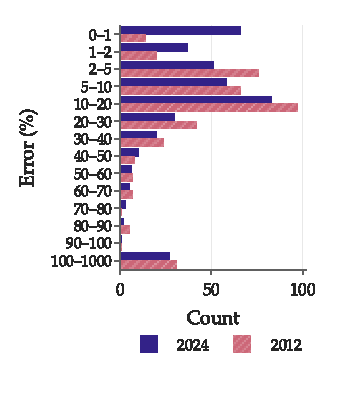
\includegraphics{figures/04/figs/acc_rt_pred_sc2023_both_Kissat_MAB_Rephases.pdf}
%         \caption{2023 Comp. Kissat\_MAB\_Rephases}
% \end{subfigure}\hfill
% \begin{subfigure}[b]{0.49\textwidth}
%         \centering
%         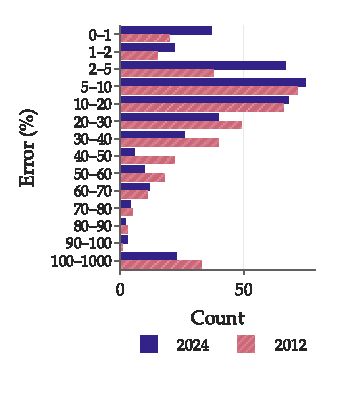
\includegraphics{figures/04/figs/acc_rt_pred_sc2023_both_Kissat_MAB_prop.pdf}
%         \caption{2023 Comp. Kissat\_MAB\_prop}
% \end{subfigure}
% \end{figure}
% \begin{figure}[p]
% \centering
% \caption[Per-solver prediction errors for SAT Competition 2023, part 5]{Per-solver running time prediction error percentages for SATZilla 2012 (rose, striped) and SATZilla 2024 (indigo).}
% \label{fig:ch04:rts_hists9}
% \begin{subfigure}[b]{0.49\textwidth}
%         \centering
%         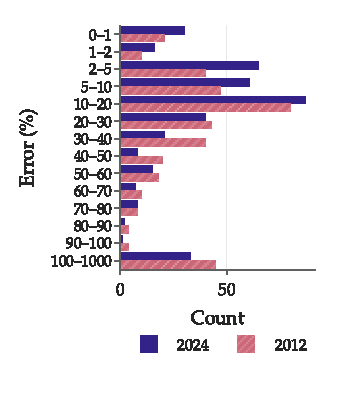
\includegraphics{figures/04/figs/acc_rt_pred_sc2023_both_Kissat_MAB_prop-no_sym.pdf}
%         \caption{2023 Comp. Kissat\_MAB\_prop-no\_sym}
% \end{subfigure}\hfill
% \begin{subfigure}[b]{0.49\textwidth}
%         \centering
%         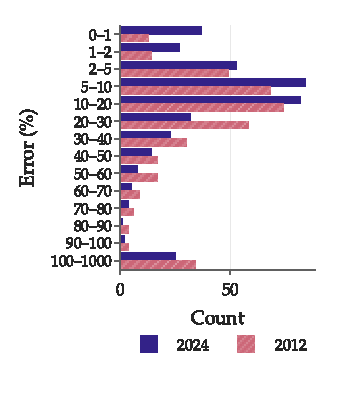
\includegraphics{figures/04/figs/acc_rt_pred_sc2023_both_Kissat_MAB_prop_pr-no_sym.pdf}
%         \caption{2023 Comp. Kissat\_MAB\_prop\_pr-no\_sym}
% \end{subfigure}
% \par\medskip
% \begin{subfigure}[b]{0.49\textwidth}
%         \centering
%         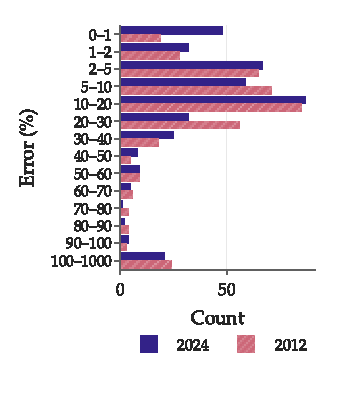
\includegraphics{figures/04/figs/acc_rt_pred_sc2023_both_MapleCaDiCaL_LBD-990_275.pdf}
%         \caption{2023 Comp. MapleCaDiCaL\_LBD-990\_275}
% \end{subfigure}\hfill
% \begin{subfigure}[b]{0.49\textwidth}
%         \centering
%         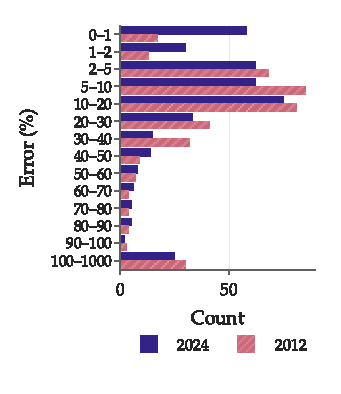
\includegraphics{figures/04/figs/acc_rt_pred_sc2023_both_MapleCaDiCaL_LBD-990_500.pdf}
%         \caption{2023 Comp. MapleCaDiCaL\_LBD-990\_500}
% \end{subfigure}
% \end{figure}
% \begin{figure}[p]
% \centering
% \caption[Per-solver prediction errors for SAT Competition 2023, part 6]{Per-solver running time prediction error percentages for SATZilla 2012 (rose, striped) and SATZilla 2024 (indigo).}
% \label{fig:ch04:rts_hists9b}
% \begin{subfigure}[b]{0.49\textwidth}
%         \centering
%         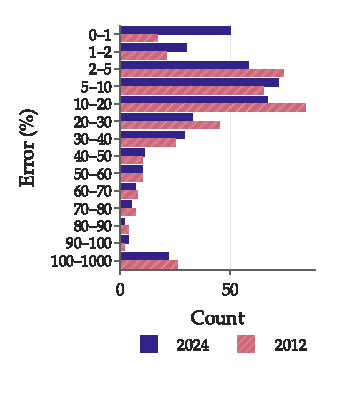
\includegraphics{figures/04/figs/acc_rt_pred_sc2023_both_MapleCaDiCaL_PPD-500_500.pdf}
%         \caption{2023 Comp. MapleCaDiCaL\_PPD-500\_500}
% \end{subfigure}\hfill
% \begin{subfigure}[b]{0.49\textwidth}
%         \centering
%         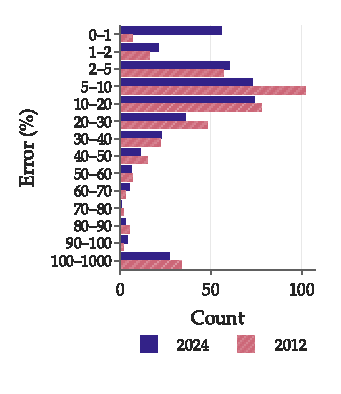
\includegraphics{figures/04/figs/acc_rt_pred_sc2023_both_MapleCaDiCaL_PPD-950_950.pdf}
%         \caption{2023 Comp. MapleCaDiCaL\_PPD-950\_950}
% \end{subfigure}
% \par\medskip
% \begin{subfigure}[b]{0.49\textwidth}
%         \centering
%         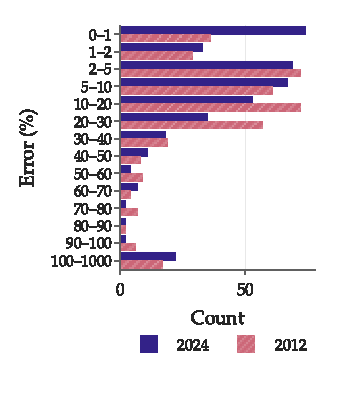
\includegraphics{figures/04/figs/acc_rt_pred_sc2023_both_MergeSat-bve_gates.pdf}
%         \caption{2023 Comp. MergeSat-bve\_gates}
% \end{subfigure}\hfill
% \begin{subfigure}[b]{0.49\textwidth}
%         \centering
%         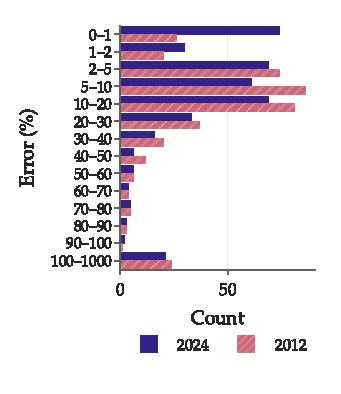
\includegraphics{figures/04/figs/acc_rt_pred_sc2023_both_MergeSat-bve_semgates.pdf}
%         \caption{2023 Comp. MergeSat-bve\_semgates}
% \end{subfigure}
% \end{figure}
% \begin{figure}[p]
% \centering
% \caption[Per-solver prediction errors for SAT Competition 2023, part 7]{Per-solver running time prediction error percentages for SATZilla 2012 (rose, striped) and SATZilla 2024 (indigo).}
% \label{fig:ch04:rts_hists10}
% \begin{subfigure}[b]{0.49\textwidth}
%         \centering
%         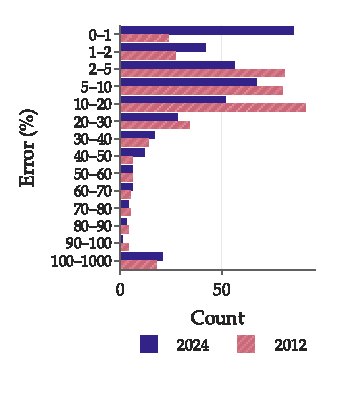
\includegraphics{figures/04/figs/acc_rt_pred_sc2023_both_MergeSat-thread1.pdf}
%         \caption{2023 Comp. MergeSat-thread1}
% \end{subfigure}\hfill
% \begin{subfigure}[b]{0.49\textwidth}
%         \centering
%         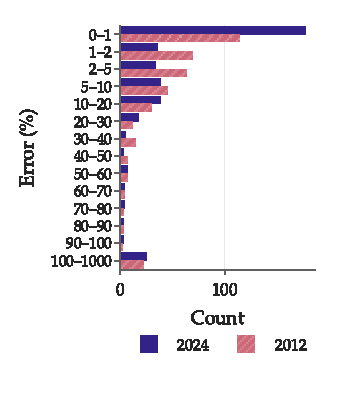
\includegraphics{figures/04/figs/acc_rt_pred_sc2023_both_MiniSat+XorEngine.pdf}
%         \caption{2023 Comp. MiniSat+XorEngine}
% \end{subfigure}
% \par\medskip
% \begin{subfigure}[b]{0.49\textwidth}
%         \centering
%         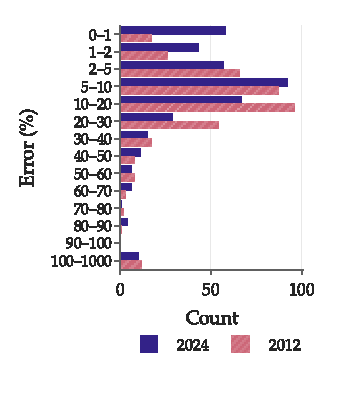
\includegraphics{figures/04/figs/acc_rt_pred_sc2023_both_PReLearn-kissat-PReLearn-kissat.sh.pdf}
%         \caption{2023 Comp. PReLearn-kissat-PReLearn-kissat.sh}
% \end{subfigure}\hfill
% \begin{subfigure}[b]{0.49\textwidth}
%         \centering
%         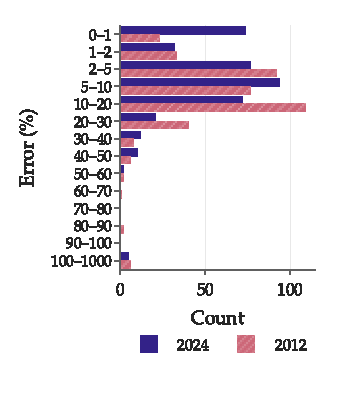
\includegraphics{figures/04/figs/acc_rt_pred_sc2023_both_PReLearn-kissat-PReLearn-tern-kissat.sh.pdf}
%         \caption{2023 Comp. PReLearn-kissat-PReLearn-tern-kissat.sh}
% \end{subfigure}
% \end{figure}
% \begin{figure}[p]
% \centering
% \caption[Per-solver prediction errors for SAT Competition 2023, part 8]{Per-solver running time prediction error percentages for SATZilla 2012 (rose, striped) and SATZilla 2024 (indigo).}
% \label{fig:ch04:rts_hists10b}
% \begin{subfigure}[b]{0.49\textwidth}
%         \centering
%         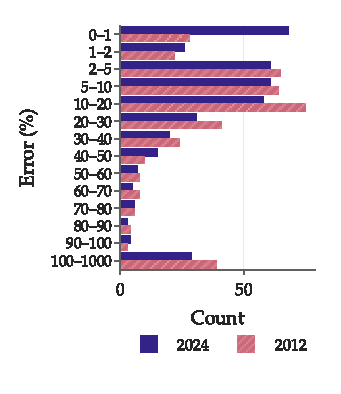
\includegraphics{figures/04/figs/acc_rt_pred_sc2023_both_ReEncode-kissat-ReEncode-pair-kissat.sh.pdf}
%         \caption{2023 Comp. ReEncode-kissat-ReEncode-pair-kissat.sh}
% \end{subfigure}\hfill
% \begin{subfigure}[b]{0.49\textwidth}
%         \centering
%         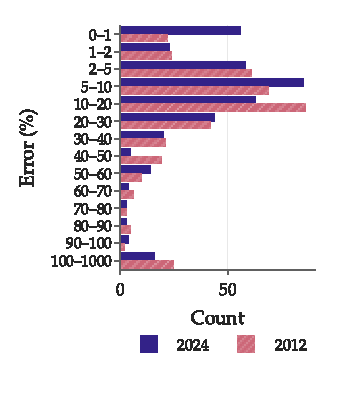
\includegraphics{figures/04/figs/acc_rt_pred_sc2023_both_SBVA-sbva_cadical.pdf}
%         \caption{2023 Comp. SBVA-sbva\_cadical}
% \end{subfigure}
% \par\medskip
% \begin{subfigure}[b]{0.49\textwidth}
%         \centering
%         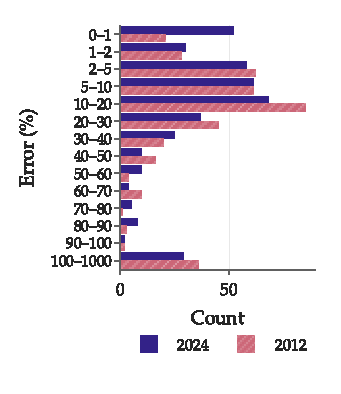
\includegraphics{figures/04/figs/acc_rt_pred_sc2023_both_SBVA-sbva_kissat.pdf}
%         \caption{2023 Comp. SBVA-sbva\_kissat}
% \end{subfigure}\hfill
% \begin{subfigure}[b]{0.49\textwidth}
%         \centering
%         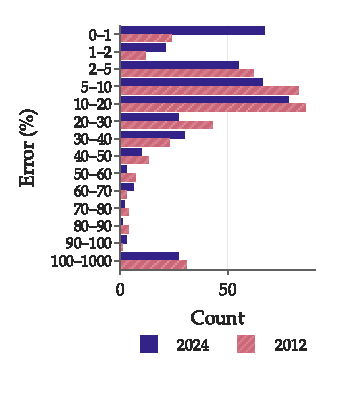
\includegraphics{figures/04/figs/acc_rt_pred_sc2023_both_SeqFROST.pdf}
%         \caption{2023 Comp. SeqFROST}
% \end{subfigure}
% \end{figure}
% \begin{figure}[p]
% \centering
% \caption[Per-solver prediction errors for SAT Competition 2023, part 9]{Per-solver running time prediction error percentages for SATZilla 2012 (rose, striped) and SATZilla 2024 (indigo).}
% \label{fig:ch04:rts_hists11}
% \begin{subfigure}[b]{0.49\textwidth}
%         \centering
%         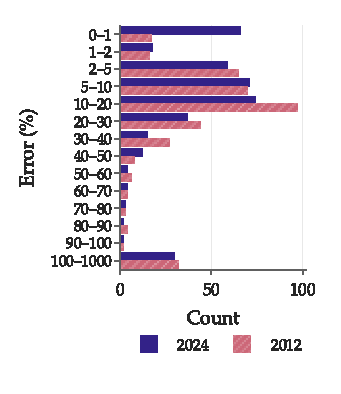
\includegraphics{figures/04/figs/acc_rt_pred_sc2023_both_SeqFROST-ERE-All.pdf}
%         \caption{2023 Comp. SeqFROST-ERE-All}
% \end{subfigure}\hfill
% \begin{subfigure}[b]{0.49\textwidth}
%         \centering
%         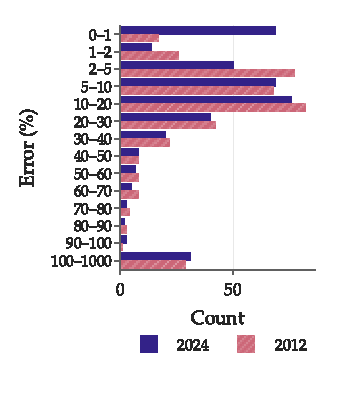
\includegraphics{figures/04/figs/acc_rt_pred_sc2023_both_SeqFROST-NoExtend.pdf}
%         \caption{2023 Comp. SeqFROST-NoExtend}
% \end{subfigure}
% \par\medskip
% \begin{subfigure}[b]{0.49\textwidth}
%         \centering
%         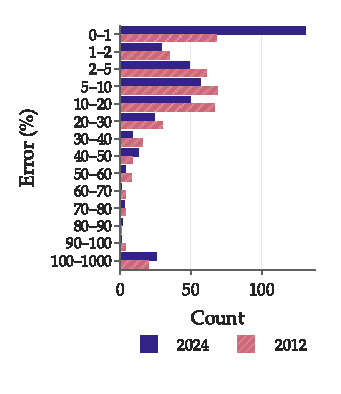
\includegraphics{figures/04/figs/acc_rt_pred_sc2023_both_hKis-psids.pdf}
%         \caption{2023 Comp. hKis-psids}
% \end{subfigure}\hfill
% \begin{subfigure}[b]{0.49\textwidth}
%         \centering
%         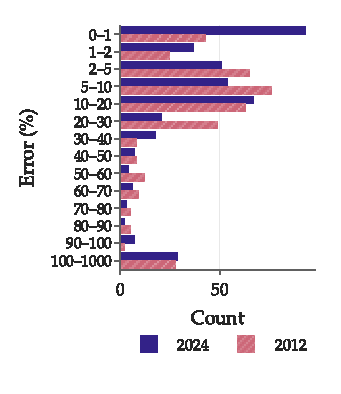
\includegraphics{figures/04/figs/acc_rt_pred_sc2023_both_hKis-sat_psids.pdf}
%         \caption{2023 Comp. hKis-sat\_psids}
% \end{subfigure}
% \end{figure}
% \begin{figure}[p]
% \centering
% \caption[Per-solver prediction errors for SAT Competition 2023, part 10]{Per-solver running time prediction error percentages for SATZilla 2012 (rose, striped) and SATZilla 2024 (indigo).}
% \label{fig:ch04:rts_hists11b}
% \begin{subfigure}[b]{0.49\textwidth}
%         \centering
%         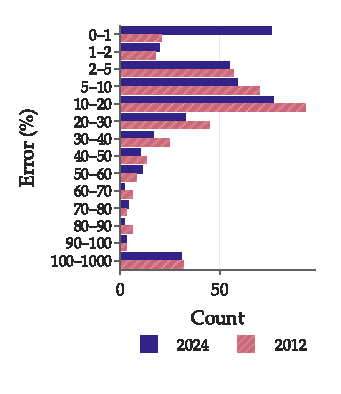
\includegraphics{figures/04/figs/acc_rt_pred_sc2023_both_hKis-unsat.pdf}
%         \caption{2023 Comp. hKis-unsat}
% \end{subfigure}\hfill
% \begin{subfigure}[b]{0.49\textwidth}
%         \centering
%         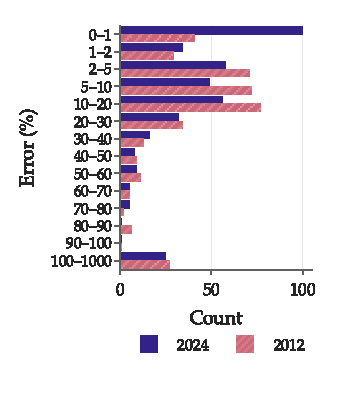
\includegraphics{figures/04/figs/acc_rt_pred_sc2023_both_hKissatInc-unsat.pdf}
%         \caption{2023 Comp. hKissatInc-unsat}
% \end{subfigure}
% \par\medskip
% \begin{subfigure}[b]{0.49\textwidth}
%         \centering
%         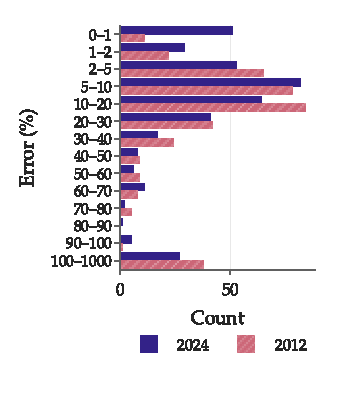
\includegraphics{figures/04/figs/acc_rt_pred_sc2023_both_kissat-3.1.0.pdf}
%         \caption{2023 Comp. kissat-3.1.0}
% \end{subfigure}\hfill
% \begin{subfigure}[b]{0.49\textwidth}
%         \centering
%         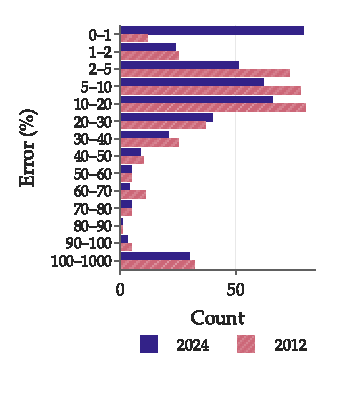
\includegraphics{figures/04/figs/acc_rt_pred_sc2023_both_kissat-hywalk-exp.pdf}
%         \caption{2023 Comp. kissat-hywalk-exp}
% \end{subfigure}
% \end{figure}
% \begin{figure}[p]
% \centering
% \caption[Per-solver prediction errors for SAT Competition 2023, part 11]{Per-solver running time prediction error percentages for SATZilla 2012 (rose, striped) and SATZilla 2024 (indigo).}
% \label{fig:ch04:rts_hists12}
% \begin{subfigure}[b]{0.49\textwidth}
%         \centering
%         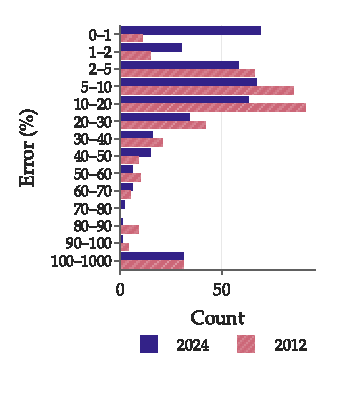
\includegraphics{figures/04/figs/acc_rt_pred_sc2023_both_kissat-hywalk-exp-gb.pdf}
%         \caption{2023 Comp. kissat-hywalk-exp-gb}
% \end{subfigure}\hfill
% \begin{subfigure}[b]{0.49\textwidth}
%         \centering
%         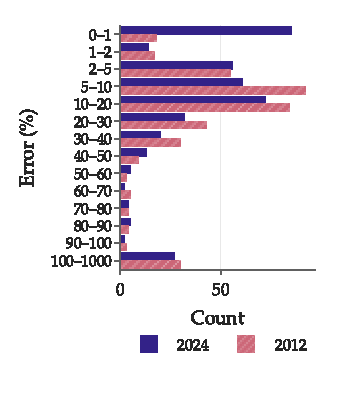
\includegraphics{figures/04/figs/acc_rt_pred_sc2023_both_kissat-hywalk-gb.pdf}
%         \caption{2023 Comp. kissat-hywalk-gb}
% \end{subfigure}
% \par\medskip
% \begin{subfigure}[b]{0.49\textwidth}
%         \centering
%         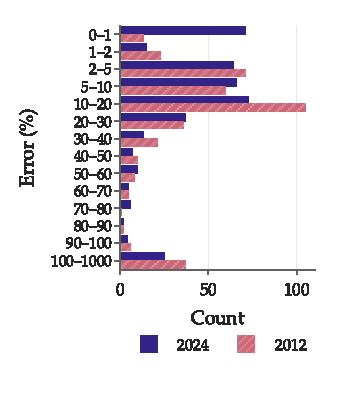
\includegraphics{figures/04/figs/acc_rt_pred_sc2023_both_kissat_incsp.pdf}
%         \caption{2023 Comp. kissat\_incsp}
% \end{subfigure}\hfill
% \begin{subfigure}[b]{0.49\textwidth}
%         \centering
%         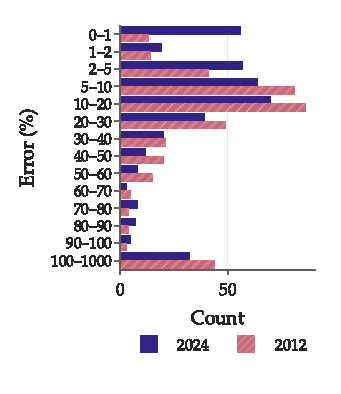
\includegraphics{figures/04/figs/acc_rt_pred_sc2023_both_tabularasat-1.0.0.pdf}
%         \caption{2023 Comp. tabularasat-1.0.0}
% \end{subfigure}
% \end{figure}
